\chapter{极限}
\section{数列极限}
\subsection{数列极限的定义}
\begin{definition}
设\(\{x_n\}\)为一数列.
如果存在常数\(a\),%
对于任意给定的正数\(\varepsilon\)(不论它多么小),%
总存在正整数\(N\),%
使得当\(n > N\)时,%
不等式\[
\abs{x_n - a} < \varepsilon
\]都成立,%
那么就称%
“数列\(\{x_n\}\)是\textbf{收敛的}(convergent)”,%
“常数\(a\)是数列\(\{x_n\}\)的\textbf{极限}”,%
或者称“数列\(\{x_n\}\)\textbf{收敛于} \(a\)”,%
记为\[
\lim\limits_{n\to\infty} x_n = a,
\]或\[
x_n \to a \quad (n \to \infty).
\]

如果不存在这样的常数\(a\),%
就说“数列\(\{x_n\}\)没有极限”,%
或者说“数列\(\{x_n\}\)是\textbf{发散的}(divergent)”,%
习惯上也说“极限\(\lim\limits_{n\to\infty} x_n\)不存在”.
\end{definition}

上面定义中正数\(\varepsilon\)可以任意给定是很重要的,因为只有这样,不等式\[
\abs{x_n - a} < \varepsilon
\]才能表达出\(x_n\)与\(a\)无限接近的意思.
此外还应注意到:
定义中的正整数\(N\)是与任意给定的正数\(\varepsilon\)有关的,它随着\(\varepsilon\)的给定而选定.

上述对数列极限的定义(即“数列\(\{a_n\}\)收敛于\(a\)”)可以简化为:\[
	\lim\limits_{n\to\infty} x_n = a
	\iff
	\forall \varepsilon > 0,
	\exists N\in\mathbb{N}^+ (n > N \implies \abs{x_n - a} < \varepsilon).
\]
而“数列\(\{a_n\}\)发散”则可表达为:\[
	\forall a \in \mathbb{R},
	\exists \varepsilon_0 > 0,
	\forall N \in \mathbb{N}^+,
	\exists n_0 > N
	(
		\abs{a_{n_0} - a} > \varepsilon_0
	).
\]


\begin{example}
证明数列\[
2,\frac{1}{2},\frac{4}{3},\frac{3}{4},\dotsc,\frac{n+(-1)^{n-1}}{n},\dotsc
\]的极限是1.
\begin{proof}
由于\[
\abs{x_n - 1}
= \abs{\frac{n+(-1)^{n-1}}{n}-1}
= \abs{\frac{(-1)^{n-1}}{n}}
= \frac{1}{n},
\]所以为使\(\abs{x_n - 1} < \varepsilon\),须取\(\frac{1}{n} < \varepsilon\)或\(\frac{1}{\varepsilon} < n\).
也就是说,对于\(\forall \varepsilon > 0\),取\(N = \floor*{\frac{1}{\varepsilon}}\),则当\(n > N\)时,就有\(\abs{x_n - a} < \varepsilon\),即\(\lim\limits_{n\to\infty}\frac{n+(-1)^{n-1}}{n}=1\).
\end{proof}
\end{example}

\begin{example}
已知\(x_n = \frac{(-1)^n}{(n+1)^2}\),证明数列\(\Set{x_n}\)的极限是\(0\).
\begin{proof}
因为\(\abs{x_n - a} = \abs{\frac{(-1)^n}{(n+1)^2}-0} = \frac{1}{(n+1)^2} < \frac{1}{n+1}\),所以对于\(\forall\varepsilon>0\)(设\(\varepsilon<1\)),只要\(\frac{1}{n+1}<\varepsilon\)或\(n>\frac{1}{\varepsilon}-1\),不等式\(\abs{x_n-a}<\varepsilon\)必定成立.所以,取\(N=\floor*{\frac{1}{\varepsilon}-1}\),则当\(n>N\)时就有\(\abs{x_n - a}<\varepsilon\),即\(\lim\limits_{n\to\infty}\frac{(-1)^n}{(n+1)^2}=0\).
\end{proof}
\end{example}

在利用数列极限的定义来论证某个数\(a\)是数列\(\{x_n\}\)的极限时,%
重要的是对于任意给定的正数\(\varepsilon\),要能够指出定义中所说的这种正整数\(N\)确实存在,%
但没有必要去求最小的\(N\).
如果知道\(\abs{x_n-a}\)小于某个量(这个量是\(n\)的一个函数),%
那么当这个量小于\(\varepsilon\)时,\(\abs{x_n-a}<\varepsilon\)当然也成立.
若令这个量小于\(\varepsilon\)来定出\(N\)比较方便的话,就可采用这种方法.

\begin{example}
设\(\abs{q}<1\),证明等比数列\[
1,q,q^2,\dotsc,q^{n-1},\dotsc
\]的极限是\(0\).
\begin{proof}
对于\(\forall\varepsilon>0\)(设\(\varepsilon<1\)),因为\(\abs{x_n-0}=\abs{q^{n-1}-0}=\abs{q}^{n-1}\),要使\(\abs{x_n-0}<\varepsilon\),只要\(\abs{q}^{n-1}<\varepsilon\).取自然对数得\((n-1)\ln\abs{q}<\ln\varepsilon\).因为\(\abs{q}<1\),\(\ln\abs{q}<0\),故\(n>1+\frac{\ln\varepsilon}{\ln\abs{q}}\).取\(N=\floor*{1+\frac{\ln\varepsilon}{\ln\abs{q}}}\),则当\(n>N\)时,就有\(\abs{q^{n-1}-0}<\varepsilon\),即
\begin{equation}
\lim\limits_{n\to\infty}q^{n-1}=0
\quad(\abs{q}<1).
\end{equation}
由此可知,当\(\abs{q}<1\)时,等比数列\(1,q,q^2,\dotsc,q^{n-1},\dotsc\)的极限是\(0\).
\end{proof}
\end{example}

\begin{example}
证明:\begin{equation}
\lim\limits_{n\to\infty} \sqrt[n]{n^k} = 1
\quad(k\in\mathbb{N}^+).
\end{equation}
\begin{proof}
要证\(\forall\varepsilon>0\),\(\exists N > 0\),使得当\(n > N\)时,
\[
\abs{\sqrt[n]{n^k} - 1} < \varepsilon.
\eqno{(1)}
\]

因为\(n \geqslant 1\),\(n^k \geqslant 1\),\(\sqrt[n]{n^k} \geqslant 1\),所以(1)式等价于\[
\abs{\sqrt[n]{n^k} - 1} = \sqrt[n]{n^k} - 1 < \varepsilon,
\]也即\(\sqrt[n]{n^k} < 1 + \varepsilon\),\(\sqrt[n]{n} < \sqrt[k]{1+\varepsilon}\),
\[
\frac{1}{n} \ln n < \frac{1}{k} \ln(1+\varepsilon);
\eqno{(2)}
\]
又因为\(\ln n < \sqrt{n}\),所以只要有\[
\frac{1}{n} \ln n < \frac{1}{n} \sqrt{n} = \frac{1}{\sqrt{n}} \leqslant \frac{1}{k} \ln(1+\varepsilon)
\]或
\[
n \geqslant \left[ \frac{k}{\ln(1+\varepsilon)} \right]^2
\eqno{(3)}
\]
成立即有(2)式成立,那么取\[
N = \ceil*{\left[ \frac{k}{\ln(1+\varepsilon)} \right]^2},
\]就对\(\forall\varepsilon>0\),\(\exists N > 0\),使得当\(n > N\)时,有\[
\abs{\sqrt[n]{n^k} - 1} < \varepsilon
\]成立.
\end{proof}
\end{example}

\subsection{收敛数列的性质}
\begin{theorem}[极限的唯一性]\label{theorem:极限.收敛数列的唯一性}
如果数列\(\{x_n\}\)收敛,那么它的极限唯一.
\begin{proof}
用反证法.
假设当\(n\to\infty\)时,同时有\(x_n \to a\)及\(x_n \to b\),且\(a < b\).
取\(\varepsilon = \frac{b-a}{2}\).
因为\(\lim\limits_{n\to\infty}x_n = a\),所以有
\[
\exists N_1 \in \mathbb{N}^+ \left(n > N_1 \implies \abs{x_n - a} < \frac{b-a}{2}\right)
\eqno{(1)}
\]
成立.
同理,因为\(\lim\limits_{n\to\infty}x_n = b\),所以有
\[
\exists N_2 \in \mathbb{N}^+ \left(n > N_2 \implies \abs{x_n - a} < \frac{b-a}{2}\right)
\eqno{(2)}
\]
成立.
取\(N = \max\{N_1,N_2\}\),则当\(n > N\)时,上述两个不等式应同时成立.
但由(1)式有\(x_n<\frac{a+b}{2}\),由(2)式有\(x_n>\frac{a+b}{2}\),矛盾,故收敛数列的极限必定唯一.
\end{proof}
\end{theorem}

\begin{example}\label{example:极限.振荡数列不存在极限}
证明数列\(x_n=(-1)^{n+1}\ (n=1,2,\dotsc)\)是发散的.
\begin{proof}
假设这级数收敛,则它具有唯一的极限\(\lim\limits_{n\to\infty}x_n = a\).
按数列极限的定义,对于\(\varepsilon=1/2\),\(\exists N \in \mathbb{N}^+\),当\(n > N\)时,\(\abs{x_n-a}<1/2\)或\(x_n\in\left(a-\frac{1}{2},a+\frac{1}{2}\right)\)成立.
但这是不可能的,因为\(n\to\infty\)时,\(x_n\)无休止地一再重复取得\(1\)和\(-1\)这两个数,而这两个数不可能同时属于长度为\(1\)的开区间\(\left(a-\frac{1}{2},a+\frac{1}{2}\right)\)内,因此这数列发散.
\end{proof}
\end{example}

\begin{definition}[数列的有界性]
对于数列\(\{x_n\}\),若\(\exists M > 0\),使得对于\(\forall x_n\)都满足不等式\[
\abs{x_n} \leqslant M,
\]则称“数列\(\{x_n\}\)是\textbf{有界的}”;
如果这样的正数\(M\)不存在,就说“数列\(\{x_n\}\)是\textbf{无界的}”.
\end{definition}
例如,数列\(x_n = \frac{n}{n+1}\ (n=1,2,\dotsc)\)是有界的,因为可取\(M=1\),而使\[
\abs{\frac{n}{n+1}} \leqslant 1
\]对于一切正整数\(n\)都成立.

数列\(x_n = 2^n\ (n=1,2,\dotsc)\)是无界的,因为当\(n\)无限增加时,\(2^n\)可超过任何正数.

\begin{theorem}[收敛数列的有界性]\label{theorem:极限.收敛数列的有界性}
如果数列\(\{x_n\}\)收敛,那么数列\(\{x_n\}\)一定有界.
\begin{proof}
既然数列\(\{x_n\}\)收敛,不妨设\(\lim\limits_{n\to\infty}x_n = a\).
根据数列极限的定义,对于\(\varepsilon = 1\),\(\exists N \in \mathbb{N}^+\),当\(n > N\)时,不等式\(\abs{x_n - a} < 1\)都成立.
于是,当\(n > N\)时,\[
\abs{x_n} = \abs{(x_n - a) + a} \leqslant \abs{x_n - a} + \abs{a} < 1 + \abs{a}.
\]
取\(M = \max\{\abs{x_1},\abs{x_2},\dotsc,\abs{x_N},1+\abs{a}\}\),%
那么数列\(\{x_n\}\)中的一切\(x_n\)都满足不等式\[
\abs{x_n} \leqslant M.
\]
这就证明了数列\(\{x_n\}\)是有界的.
\end{proof}
\end{theorem}

根据\cref{theorem:极限.收敛数列的有界性} 立即有以下推论.
\begin{corollary}
如果数列\(\{x_n\}\)是无界的,那么数列\(\{x_n\}\)一定发散.
\end{corollary}
但是,如果数列\(\{x_n\}\)有界,却不能断定数列\(\{x_n\}\)一定收敛.
例如,在\cref{example:极限.振荡数列不存在极限} 中,数列\[
1,-1,1,\dotsc,(-1)^{n+1},\dotsc
\]有界,但它是发散的.
于是我们可以说:数列有界是数列收敛的必要不充分条件.

\begin{theorem}[收敛数列的保号性]\label{theorem:极限.收敛数列的保号性}
如果\(\lim\limits_{n\to\infty}x_n = a\),且\(a \gtrless 0\),那么\(\exists N \in \mathbb{N}^+\),当\(n > N\)时,都有\(x_n \gtrless 0\).
\begin{proof}
当\(a > 0\)时,由数列极限的定义,对\(\varepsilon = \frac{a}{2} > 0\),\(\exists N \in \mathbb{N}^+\),当\(n > N\)时,有\(\abs{x_n - a} < \frac{a}{2}\),从而\(x_n > a - \frac{a}{2} = \frac{a}{2} > 0\).
同样地,当\(a < 0\)时,对\(\varepsilon = -\frac{a}{2} > 0\),\(\exists N \in \mathbb{N}^+\),当\(n > N\)时,有\(\abs{x_n - a} < -\frac{a}{2}\),从而\(x_n < a - \frac{a}{2} = \frac{a}{2} < 0\).
\end{proof}
\end{theorem}

\begin{corollary}
如果数列\(\{x_n\}\)从某项起有\(x_n \geqslant 0\)(或\(x_n \leqslant 0\)),且\(\lim\limits_{n\to\infty}x_n = a\),那么\(a \geqslant 0\)(或\(a \leqslant 0\)).
\begin{proof}
设当\(n > N_1\)(\(N_1 \in \mathbb{N}^+\))时有\(x_n \geqslant 0\).用反证法.假设\(\lim\limits_{n\to\infty}x_n = a < 0\),则由收敛数列的保号性定理可知,\(\exists N_2 \in \mathbb{N}^+\),当\(n > N_2\)时,有\(x_n < 0\).取\(N = \max\{N_1,N_2\}\),当\(n > N\)时,按假定有\(x_n \geqslant 0\),又由保号性可得\(x_n < 0\),这引起矛盾,所以必有\(a \geqslant 0\).
\end{proof}
\end{corollary}

\begin{example}
\def\l{\lim\limits_{n\to\infty}}
\def\ys{\l \frac{\sqrt{n^2+a^2}}{n}}
根据数列极限的定义证明:\(\ys = 1\).
\begin{proof}[证法1]
记\(x_n = \frac{\sqrt{n^2+a^2}}{n}\).
\(\abs{x_n-1} = \abs{\frac{\sqrt{n^2+a^2}}{n}-1} = \frac{\sqrt{n^2+a^2}-n}{n}\).

当\(a > 0\)时,\((n+a)^2-(n^2+a^2)=2an>0\),\(\sqrt{n^2+a^2}<\sqrt{(n+a)^2}=n+a\),\(\frac{\sqrt{n^2+a^2}-n}{n} < \frac{n+a-n}{n} = \frac{a}{n}\);

当\(a < 0\)时,\((n-a)^2-(n^2+a^2)=-2an>0\),\(\sqrt{n^2+a^2}<\sqrt{(n-a)^2}=\abs{n-a}\),\(\frac{\sqrt{n^2+a^2}-n}{n} < \frac{\abs{n-a}-n}{n} \leqslant \frac{\abs{(n-a)-n}}{n} = \frac{a}{n}\);

当\(a = 0\)时,\(\frac{\sqrt{n^2+a^2}-n}{n} = \frac{\sqrt{n^2}-n}{n} = 0\).

对于\(\forall\varepsilon>0\),要使\(\abs{x_n-1}<\varepsilon\),根据上面的讨论可知,只需\(\frac{a}{n}<\varepsilon\),\(n>\frac{a}{\varepsilon}\).
取\(N = \floor*{\frac{a}{\varepsilon}}\),则当\(n>N\)时有\(\abs{x_n-1}<\varepsilon\),即\[
\ys = 1.
\qedhere
\]
\end{proof}
\begin{proof}[证法2]
依然记\(x_n = \frac{\sqrt{n^2+a^2}}{n}\).这里运用分子有理化方法简化\(\abs{x_n-1}\).
\begin{align*}
\abs{x_n-1} &= \abs{\frac{\sqrt{n^2+a^2}}{n}-1}
= \frac{\sqrt{n^2+a^2}-n}{n}
= \frac{(n^2+a^2)-n^2}{n (\sqrt{n^2+a^2}+n)} \\
&= \frac{a^2}{n (\sqrt{n^2+a^2}+n)}
\leqslant \frac{a^2}{n^2}.
\end{align*}

对于\(\forall\varepsilon>0\),要使\(\abs{x_n-1}<\varepsilon\),只需\(\frac{a^2}{n^2}<\varepsilon\),\(n^2>\frac{a^2}{\varepsilon}\),\(n>\sqrt\frac{a^2}{\varepsilon}\).
取\(N = \floor*{\sqrt\frac{a^2}{\varepsilon}}\),则当\(n>N\)时有\(\abs{x_n-1}<\varepsilon\),即\[
\ys = 1.
\qedhere
\]
\end{proof}
\end{example}

\begin{example}
\def\l{\lim\limits_{n\to\infty}}
\def\ys{\l 0.\underbrace{999\cdots9}_{n\text{个}}}
根据数列极限的定义证明:\(\ys = 1\).
\begin{proof}
记\(x_n = 1-\frac{1}{10^n}\).
\(\abs{x_n - 1} = \abs{\left(1-\frac{1}{10^n}\right)-1} = \frac{1}{10^n}\).

对\(\forall \varepsilon>0\)(设\(\varepsilon<1\)),要使\(\abs{x_n-1}<\varepsilon\),只需\(\frac{1}{10^n}<\varepsilon\),\(10^n>\frac{1}{\varepsilon}\),\(n>\lg\frac{1}{\varepsilon}=-\lg\varepsilon\).
取\(N=\floor{-\lg\varepsilon}\),则当\(n>N\)时有\(\abs{x_n-1}<\varepsilon\)成立,即\[
\l x_n = \l \left(1-\frac{1}{10^n}\right) = \ys = 1.
\qedhere
\]
\end{proof}
\end{example}

\begin{example}
\def\l{\lim\limits_{n\to\infty}}
设数列\(\{x_n\}\)有界,又\(\l y_n = 0\),证明:\(\l x_n y_n = 0\).
\begin{proof}
由数列\(\{x_n\}\)有界,\(
\exists M > 0, \forall x_n (\abs{x_n} \leqslant M)
\).

因为\(\l y_n = 0\),所以对\(\forall \varepsilon > 0\),\(\exists N_0 \in \mathbb{N}^+\),使得当\(n>N_0\)时,\(\abs{y_n - 0} = \abs{y_n} < \frac{\varepsilon}{M}\)成立,进而有\[
\abs{x_n y_n - 0} = \abs{x_n y_n} = \abs{x_n} \abs{y_n} < M \cdot \frac{\varepsilon}{M} = \varepsilon.
\qedhere
\]
\end{proof}
\end{example}

\subsection{子列极限与上下极限}
上、下极限是数列极限的必要组成部分,它们各有三种等价的描述方式,或者说三种等价的定义.给定一种定义后,其余两种定义的内容可以命题或定理的形式得到证明.
\begin{definition}
在数列\(\{x_n\}\)中任意抽取无限多项并保持这些项在原数列\(\{x_n\}\)中的先后次序,这样得到的一个数列\[
x_{p_1},x_{p_2},\dotsc,x_{p_n},\dotsc
\quad(1 \leqslant p_1 < p_2 < \dotsb)
\]称为原数列\(\{x_n\}\)的\DefineConcept{子数列}(或\DefineConcept{子列}).

若子列\(\{x_{p_n}\}\)满足\[
\lim\limits_{n\to\infty} x_{p_n} = \xi,
\]则称数\(\xi\)为数列\(\{x_n\}\)的\DefineConcept{子列极限}(或极限点、聚点).

数列\(\{x_n\}\)的最小子列极限称为此数列的\DefineConcept{下极限},记作\[
\varliminf\limits_{n\to\infty} x_n.
\]

数列\(\{x_n\}\)的最大子列极限称为此数列的\DefineConcept{上极限},记作\[
\varlimsup\limits_{n\to\infty} x_n.
\]
\end{definition}
上面对上下极限的定义可以利用“\(\varepsilon-N\)语言”更加简洁精确地重新定义为\begin{align*}
\varliminf\limits_{n\to\infty} x_n = \alpha \in (-\infty,+\infty)
&\iff \forall\varepsilon>0, \exists N\in\mathbb{N}^+ \bigl( n>N \implies \alpha-\varepsilon < x_n \bigr); \\
\varlimsup\limits_{n\to\infty} x_n = \beta \in (-\infty,+\infty)
&\iff \forall\varepsilon>0, \exists N\in\mathbb{N}^+ \bigl( n>N \implies x_n < \beta+\varepsilon \bigr).
\end{align*}

\begin{theorem}[波尔查诺-魏尔斯特拉斯原理]\label{theorem:极限.波尔查诺-魏尔斯特拉斯原理}
任何有界数列至少有一个有限的子列极限.
\end{theorem}

\begin{theorem}\label{theorem:极限.上下极限的等价定义1}
数列\(\{x_n\}\)的上下极限满足:\[
\varliminf\limits_{n\to\infty} x_n = \lim\limits_{n\to\infty} \inf\{x_n,x_{n+1},\dotsc\},
\]\[
\varlimsup\limits_{n\to\infty} x_n = \lim\limits_{n\to\infty} \sup\{x_n,x_{n+1},\dotsc\}.
\]
\end{theorem}
这也是数列的上下极限的一种等价定义.

\begin{theorem}[收敛数列与其子列的关系]
如果数列\(\{x_n\}\)收敛于\(a\),那么它的任一子列也收敛,且极限也是\(a\).即\[
\lim\limits_{n\to\infty} x_n = a
\iff
\varliminf\limits_{n\to\infty} x_n = \varlimsup\limits_{n\to\infty} x_n = a.
\]
\begin{proof}
设数列\(\{x_{n_k}\}\)是数列\(\{x_n\}\)的任一子数列.由于\(\lim\limits_{n\to\infty}x_n = a\),故\(\forall \varepsilon > 0\),\(\exists N \in \mathbb{N}^+\),当\(n > N\)时,\(\abs{x_n - a} < \varepsilon\)成立.取\(K = N\),则当\(k > K\)时,由\(n_k > n_K \geqslant N\)得\(\abs{x_{n_k} - a} < \varepsilon\),也就是说\(\lim\limits_{k\to\infty}x_{n_k} = a\).
\end{proof}
\end{theorem}
由此可知,如果数列\(\{x_n\}\)的两个子列收敛于不同的极限,那么数列\(\{x_n\}\)是发散的.
例如数列\(\{x_n=(-1)^{n+1}\}\)的子数列\(\{x_{2k-1}\}\)收敛于\(1\),而其子数列\(\{x_{2k}\}\)收敛于\(-1\),因此数列\(\{x_n\}\)是发散的.
同时这个例子也说明,一个发散的数列也可能有收敛的子数列.

\begin{example}
\def\l{\lim\limits_{n\to\infty}}
若\(\l u_n = a\),证明\(\l \abs{u_n} = \abs{a}\).并举例说明:如果数列\(\{\abs{x_n}\}\)有极限,但数列\(\{x_n\}\)未必有极限.
\begin{proof}
因为\(\l u_n = a\),所以对\(\forall\varepsilon>0\),\(\exists N \in \mathbb{N}^+\),使得当\(n>N\)时,有\(\abs{u_n-a}<\varepsilon\)成立.
根据三角不等式有\(\abs{\abs{u_n}-\abs{a}} \leqslant \abs{u_n-a}\),显然当\(n>N\)时,也有\(\abs{\abs{u_n}-\abs{a}}<\varepsilon\)成立,即\(\l \abs{u_n} = \abs{a}\).

根据前面的例子,数列\(x_n = (-1)^{n+1}\)发散,但\(\abs{x_n} = \abs{(-1)^{n+1}} = 1\)收敛,说明如果数列\(\{\abs{x_n}\}\)有极限,但数列\(\{x_n\}\)未必有极限.
\end{proof}
\end{example}

\begin{example}
\def\l#1{\lim\limits_{#1\to\infty}}
对于数列\(\{x_n\}\),若\(\l{k}x_{2k-1}=a\),\(\l{k}x_{2k}=a\),证明:\(\l{n}x_n=a\).
\begin{proof}
因为\(\l{k}x_{2k-1}=a\),所以对于\(\forall\varepsilon>0\),\(\exists N_1 \in \mathbb{N}^+\),当\(k>N_1\)时,有\(\abs{x_{2k-1}-a}<\varepsilon\)成立.

因为\(\l{k}x_{2k}=a\),所以对于\(\forall\varepsilon>0\),\(\exists N_2 \in \mathbb{N}^+\),当\(k>N_2\)时,有\(\abs{x_{2k}-a}<\varepsilon\)成立.

对于\(\forall\varepsilon>0\),取\(N = \max\{N_1,N_2\}\),当\(k>N\)时,同时有\[
\abs{x_{2k-1}-a}<\varepsilon, \qquad \abs{x_{2k}-a}<\varepsilon
\]即\[
a-\varepsilon<x_{2k-1}<a+\varepsilon, \qquad a-\varepsilon<x_{2k}<a+\varepsilon
\]成立,那么当\(n>N\)时,\(a-\varepsilon<x_n<a+\varepsilon\)或\(\abs{x_n-a}<\varepsilon\)成立,也就是说\(\l{n}x_n=a\).
\end{proof}
\end{example}

\section{函数极限}
从\hyperref[definition.数列.数列的定义]{数列的定义}可以看出,%
任意一个数列\(\{x_n\}\)只不过是一个以\(n\)为自变量的函数\(x_n = f(n)\).
我们只要把数列极限概念中“自变量\(n\)的取值范围是整数的子集”“自变量变化过程是\(n\to\infty\)”等特殊性撇开,%
就可以引出函数极限的一般概念.

\subsection{函数极限的定义}
\subsubsection*{自变量趋于有限值时函数的极限}
\begin{definition}\label{definition:极限.函数极限的定义1}
设函数\(f(x)\)在点\(x_0\)的某一去心邻域内有定义.
如果存在常数\(A\),%
对于任意给定的正数\(\varepsilon\)(不论它多么小),%
总存在正数\(\delta\),%
使得当\(x\)满足不等式\(0 < \abs{x-x_0} < \delta\)时,%
对应的函数值\(f(x)\)都满足不等式\(\abs{f(x)-A}<\varepsilon\),%
那么常数\(A\)就叫做“函数\(f(x)\)当\(x \to x_0\)时的\textbf{极限}”,%
记作
\[
\lim\limits_{x \to x_0} f(x) = A
\quad\text{或}\quad
f(x) \to A\ (x \to x_0).
\]
\end{definition}

上述对函数极限的定义可以简化为:
\[
\lim\limits_{x \to x_0}f(x) = A
\iff
\forall \varepsilon > 0,
\exists \delta > 0
\bigl( 0 < \abs{x - x_0} < \delta \implies \abs{f(x) - A} < \varepsilon \bigr).
\]

现在我们来根据定义尝试计算一些函数的极限.
\begin{example}
证明:\(\lim\limits_{x \to x_0} c = c\),其中\(c\)为常数.
\begin{proof}
这里\(\abs{f(x) - A} = \abs{c - c} = 0\),因此\(\forall \varepsilon > 0\),可任取\(\delta > 0\),当\(0 < \abs{x - x_0} < \delta\)时,总能使不等式\[
\abs{f(x) - A} = \abs{c - c} = 0 < \varepsilon
\]成立,所以\(\lim\limits_{x \to x_0} c = c\).
\end{proof}
\end{example}

\begin{example}
证明:\(\lim\limits_{x \to x_0} x = x_0\).
\begin{proof}
这里\(\abs{f(x) - A} = \abs{x - x_0}\),因此\(\forall \varepsilon > 0\),总可取\(\delta = \varepsilon\),当\(0 < \abs{x - x_0} < \delta = \varepsilon\)时,能使不等式\(\abs{f(x) - A} = \abs{x - x_0} < \varepsilon\)成立,所以\(\lim\limits_{x \to x_0} x = x_0\).
\end{proof}
\end{example}

\begin{example}
证明:\(\lim\limits_{x\to1} 2x-1 = 1\).
\begin{proof}
由于\(\abs{f(x) - A} = \abs{(2x-1) - 1} = 2\abs{x-1}\),为了使\(\abs{f(x) - A} < \varepsilon\),只要\(\abs{x-1}<\varepsilon/2\).因此\(\forall \varepsilon > 0\),可取\(\delta = \varepsilon/2\),则当\(x\)适合不等式\[
0 < \abs{x-1} < \delta = \frac{\varepsilon}{2}
\]时,对应的函数值\(f(x)\)就满足不等式\[
\abs{f(x) - 1} = \abs{(2x-1) - 1} = 2\abs{x-1} < \varepsilon.
\]从而\(\lim\limits_{x\to1} 2x-1 = 1\).
\end{proof}
\end{example}

\begin{example}
证明:\(\lim\limits_{x\to1} \frac{x^2-1}{x-1} = 2\).
\begin{proof}
这里,函数在点\(x=1\)处是没有定义的,但是函数当\(x\to1\)时的极限存在或不存在与之无关.事实上,\(\forall \varepsilon > 0\),将不等式\[
\abs{\frac{x^2-1}{x-1} - 2} < \varepsilon
\]约去非零因子\(x-1\)后,就化为\[
\abs{(x+1)-2} = \abs{x-1} < \varepsilon,
\]因此,只要取\(\delta = \varepsilon\),那么当\(0 < \abs{x-1} < \delta\)时,就有\[
\abs{\frac{x^2-1}{x-1} - 2} < \varepsilon.
\]所以\(\lim\limits_{x\to1} \frac{x^2-1}{x-1} = 2\).
\end{proof}
\end{example}

\begin{example}
证明:当\(x_0 > 0\)时,\(\lim\limits_{x \to x_0}\sqrt{x} = \sqrt{x_0}\).
\begin{proof}
\(\forall \varepsilon > 0\),因为\[
\abs{f(x) - A} = \abs{\sqrt{x} - \sqrt{x_0}}
= \abs{\frac{x - x_0}{\sqrt{x} + \sqrt{x_0}}}
\leqslant \frac{\abs{x - x_0}}{\sqrt{x_0}},
\]要使\(\abs{f(x) - A} < \varepsilon\),只要\(\abs{x - x_0} < \sqrt{x_0} \varepsilon\).
因为\(f(x)\)在\(x_0\)的去心领域要有定义,所以\(x \geqslant 0\);而\(x \geqslant 0\)可用\(\abs{x - x_0} < x_0\)保证.
因此取\(\delta = \min\{x_0,\sqrt{x_0} \varepsilon\}\),则当\(0 < \abs{x - x_0} < \delta\)时,对应的函数值\(\sqrt{x}\)就满足\[
\abs{f(x) - A} = \abs{\sqrt{x} - \sqrt{x_0}} < \varepsilon,
\]所以\(\lim\limits_{x \to x_0}\sqrt{x} = \sqrt{x_0}\).
\end{proof}
\end{example}

\begin{definition}\label{definition:极限.函数极限的定义2}
设函数\(f(x)\)在\(x < x_0\)时有定义.
如果存在常数\(A\),%
对于任意给定的正数\(\varepsilon\),%
总存在正数\(\delta\),%
使得当\(x\)满足不等式\(-\delta < x - x_0 < 0\)或\(x_0 - \delta < x < x_0\)时,%
对应的函数值\(f(x)\)都满足不等式\(\abs{f(x) - A} < \varepsilon\),%
那么常数\(A\)就叫做“函数\(f(x)\)当\(x \to x_0\)时的\textbf{左极限}”,%
记作\[
\lim\limits_{x \to x_0^-} f(x) = A
\quad\text{或}\quad
f(x_0^-) = A.
\]
\end{definition}

\begin{definition}\label{definition:极限.函数极限的定义3}
设函数\(f(x)\)在\(x > x_0\)时有定义.
如果存在常数\(A\),%
对于任意给定的正数\(\varepsilon\),%
总存在正数\(\delta\),%
使得当\(x\)满足不等式\(0 < x - x_0 < \delta\)或\(x_0 < x < x_0 + \delta\)时,%
对应的函数值\(f(x)\)都满足不等式\(\abs{f(x) - A} < \varepsilon\),%
那么常数\(A\)就叫做“函数\(f(x)\)当\(x \to x_0\)时的\textbf{右极限}”,%
记作\[
\lim\limits_{x \to x_0^+} f(x) = A
\quad\text{或}\quad
f(x_0^+) = A.
\]
\end{definition}
左极限与右极限统称为\textbf{单侧极限}.

\begin{theorem}
函数\(f(x)\)当\(x \to x_0\)时极限存在的充要条件是:其左极限和右极限分别存在且相等,即\[
f(x_0^-) = f(x_0^+).
\]
\end{theorem}

\begin{example}
证明:函数\[
f(x) = \left\{ \begin{array}{lc}
x-1, & x<0, \\
0, & x=0, \\
x+1, & x>0.
\end{array} \right.
\]当\(x\to0\)时\(f(x)\)的极限不存在.
\begin{proof}
易证\[
\lim\limits_{x\to0^-} f(x) = \lim\limits_{x\to0^-} x-1 = -1,
\]而\[
\lim\limits_{x\to0^+} f(x) = \lim\limits_{x\to0^+} x+1 = 1,
\]因为左、右极限存在但不相等,所以\(\lim\limits_{x\to0}\)不存在.
\end{proof}
\end{example}

\subsubsection*{自变量趋于无穷大时函数的极限}
\begin{definition}\label{definition:极限.函数极限的定义4}
设函数\(f(x)\)当\(\abs{x}\)大于某一正数时有定义.
如果存在常数\(A\),%
对于任意给定的正数\(\varepsilon\)(不论它多么小),%
总存在正数\(X\),%
使得当\(x\)满足不等式\(\abs{x} > X\)时,%
对应的函数值\(f(x)\)都满足不等式\[
\abs{f(x) - A} < \varepsilon,
\]那么常数\(A\)就叫做“函数\(f(x)\)当\(x \to \infty\)时的\textbf{极限}”,%
记作\[
\lim\limits_{x \to \infty} f(x) = A
\quad\text{或}\quad
f(\infty) = A
\quad\text{或}\quad
f(x) \to A\ (x \to \infty).
\]
\end{definition}
\cref{definition:极限.函数极限的定义4} 可以简化为:
\[
\lim\limits_{x\to\infty} f(x) = A
\iff
\forall\varepsilon>0,
\exists X>0
\bigl(
	\abs{x} > X
	\implies
	\abs{f(x) - A} < \varepsilon
\bigr).
\]

我们只要对\cref{definition:极限.函数极限的定义4} 中的条件稍加改变,%
就可以得到以下两种不同的极限定义.
\begin{definition}\label{definition:极限.函数极限的定义5}
设函数\(f(x)\)在\(x > 0\)时有定义.
如果存在常数\(A\),%
对于任意给定的正数\(\varepsilon\),%
总存在正数\(X\),%
使得当\(x\)满足不等式\(x > X\)时,%
对应的函数值\(f(x)\)都满足不等式\[
\abs{f(x) - A} < \varepsilon,
\]那么常数\(A\)就叫做“函数\(f(x)\)当\(x \to +\infty\)时的\textbf{极限}”,%
记作\[
\lim\limits_{x \to +\infty} f(x) = A
\quad\text{或}\quad
f(+\infty) = A
\quad\text{或}\quad
f(x) \to A\ (x \to +\infty).
\]
\end{definition}

\begin{definition}\label{definition:极限.函数极限的定义6}
设函数\(f(x)\)在\(x < 0\)时有定义.
如果存在常数\(A\),%
对于任意给定的正数\(\varepsilon\),%
总存在正数\(X\),%
使得当\(x\)满足不等式\(x < -X\)时,%
对应的函数值\(f(x)\)都满足不等式\[
\abs{f(x) - A} < \varepsilon,
\]那么常数\(A\)就叫做“函数\(f(x)\)当\(x \to -\infty\)时的\textbf{极限}”,%
记作\[
\lim\limits_{x \to -\infty} f(x) = A
\quad\text{或}\quad
f(-\infty) = A
\quad\text{或}\quad
f(x) \to A\ (x \to -\infty).
\]
\end{definition}

\begin{example}
\def\l{\lim\limits_{x\to\infty}}
证明:\(\l \frac{1}{x} = 0\).
\begin{proof}
\(\forall\varepsilon>0\),要证\(\exists X > 0\),当\(\abs{x}>X\)时,不等式\[
\abs{\frac{1}{x}-0}<\varepsilon
\]成立.
因这个不等式相当于\(\frac{1}{\abs{x}}<\varepsilon\)或\(\abs{x}>\frac{1}{\varepsilon}\).
由此可知,如果取\(X=\frac{1}{\varepsilon}\),%
那么当\(\abs{x}>X=\frac{1}{\varepsilon}\)时,%
不等式\(\abs{\frac{1}{x}-0}<\varepsilon\)成立,%
这就证明了\(\l \frac{1}{x} = 0\).
\end{proof}
\end{example}

\subsection{函数极限的性质}
与收敛数列的性质相比较,可得函数极限的一些相应的性质.它们都可以根据函数极限的定义,运用类似于证明收敛数列性质的方法加以证明.由于函数极限的定义按自变量的变化过程不同有各种形式,下面仅以“\(\lim\limits_{x \to x_0}f(x)\)”这种形式为代表给出关于函数极限性质的一些定理,并就其中的几个给出证明.至于其他形式的极限的性质及其证明,只要相应地做一些修改即可得出.

\begin{theorem}[函数极限的唯一性]\label{theorem:极限.函数极限的唯一性}
如果\(\lim\limits_{x \to x_0}f(x)\)存在,那么这极限唯一.
\end{theorem}

\begin{theorem}[函数极限的局部有界性]\label{theorem:极限.函数极限的局部有界性}
如果\(\lim\limits_{x \to x_0}f(x) = A\),那么存在常数\(M>0\)和\(\delta>0\),%
使得当\(0<\abs{x-x_0}<\delta\)时,有\(\abs{f(x)} \leqslant M\).
\begin{proof}
因为\(\lim\limits_{x \to x_0}f(x) = A\),所以若取\(\varepsilon = 1\),则\(\exists \delta > 0\),当\(0 < \abs{x - x_0} < \delta\)时,有\[
\abs{f(x) - A} < 1 \implies \abs{f(x)} \leqslant \abs{f(x) - A} + \abs{A} < \abs{A} + 1.
\]记\(M = \abs{A} + 1\)即可.
\end{proof}
\end{theorem}

\begin{theorem}[函数极限的局部保号性]\label{theorem:极限.函数极限的局部保号性1}
如果\(\lim\limits_{x \to x_0}f(x)=A\),且\(A \gtrless 0\),那么存在常数\(\delta>0\),使得当\(0<\abs{x-x_0}<\delta\)时,有\(f(x) \gtrless 0\).
\begin{proof}
就\(A > 0\)的情形证明.因为\(\lim\limits_{x \to x_0}f(x) = A > 0\),所以若取\(\varepsilon = \frac{A}{2} > 0\),则\(\exists \delta > 0\),当\(0 < \abs{x - x_0} < \delta\)时,有\[
\abs{f(x) - A} < \varepsilon = \frac{A}{2}
\implies f(x) > A - \frac{A}{2} = \frac{A}{2} > 0.
\]类似地可以证明\(A < 0\)的情形.
\end{proof}
\end{theorem}

\begin{theorem}\label{theorem:极限.函数极限的局部保号性2}
如果\(\lim\limits_{x \to x_0}f(x) = A \neq 0\),那么就存在着\(x_0\)的某一去心邻域\(\mathring{U}(x_0)\),当\(x\in\mathring{U}(x_0)\)时,就有\(\abs{f(x)}>\frac{\abs{A}}{2}\).
\end{theorem}

\begin{corollary}\label{theorem:极限.函数极限的局部保号性3}
如果在\(x_0\)的某去心邻域内\(f(x) \geqslant 0\)(或\(f(x) \leqslant 0\)),而且\(\lim\limits_{x \to x_0}f(x) = A\),那么\(A \geqslant 0\)(或\(A \leqslant 0\)).
\end{corollary}

\begin{example}
设函数\(f(x)\)在区间\((0,+\infty)\)上单调减少,证明:若\[
\lim\limits_{x\to+\infty}f(x)=A,
\]则\(f(x)>A\)恒成立.
\begin{proof}
假设\[
\exists x_0 > 0 \bigl[
	f(x_0) < A
\bigr],
\]那么\[
\forall x > x_0 \bigl[
	f(x) < f(x_0) < A
\bigr].
\]而\[
f(x) - A < f(x_0) - A < 0
\implies
\abs{f(x) - A} > \abs{f(x_0) - A} > 0,
\]所以\[
\forall x > x_0 \bigl[
	\abs{f(x) - A} > \abs{f(x_0) - A} > 0
\bigr].
\]而这又与\[
\lim\limits_{x\to+\infty}f(x)=A
\iff
\forall \varepsilon > 0, \exists X > 0 \bigl[
	x > X \implies \abs{f(x) - A} < \varepsilon
\bigr]
\]矛盾,说明\(\forall x_0 > 0 \bigl[
	f(x_0) > A
\bigr]\).
\end{proof}
\end{example}

\begin{theorem}[函数极限的保序性]\label{theorem:极限.函数极限的保序性}
若函数\(f(x)\)和\(g(x)\)在区间\(I\)上满足\(f(x) \leqslant g(x)\),那么有\[
\varlimsup\limits_{x \to a} f(x) \leqslant \varlimsup\limits_{x \to a} g(x),
\]\[
\varliminf\limits_{x \to a} f(x) \leqslant \varliminf\limits_{x \to a} g(x).
\]
\end{theorem}

\begin{example}
\def\l{\lim\limits_{n\to+\infty}}
根据函数极限的定义证明:\(\l\frac{\sin x}{\sqrt x} = 0\).
\begin{proof}
\(\forall \varepsilon>0\),要证\(\exists X > 0\),当\(x > X\)时,不等式\[
\abs{\frac{\sin x}{\sqrt x} - 0} = \frac{\abs{\sin x}}{\sqrt x}
\leqslant \frac{1}{\sqrt x} < \varepsilon
\]成立.因这个不等式相当于\(\sqrt x > 1/\varepsilon\)或\(x > 1/\varepsilon^2\),由此可知,如果取\(X = 1/\varepsilon^2\),那么当\(x > X = \frac{1}{\varepsilon^2}\)时,不等式\(\abs{\frac{\sin x}{\sqrt x} - 0} < \varepsilon\)成立,这就证明了\(\l\frac{\sin x}{\sqrt x} = 0\).
\end{proof}
\end{example}

\begin{example}
\def\l#1{\lim\limits_{x\to#1}}
证明:\(\l0\abs{x}=0\).
\begin{proof}
先证\(\l{0^+}\abs{x}=0\).
\(\forall \varepsilon>0\),要证\(\exists \delta > 0\),当\(0<x<\delta\)时,不等式\[
\abs{\abs{x} - 0} = x < \varepsilon
\]成立,只需令\(\delta = \varepsilon\)即可.

再证\(\l{0^-}\abs{x}=0\).
\(\forall \varepsilon>0\),要证\(\exists \delta > 0\),当\(-\delta<x<0\)时,不等式\[
\abs{\abs{x} - 0} = -x < \varepsilon
\quad \text{或} \quad
x > -\varepsilon
\]成立,只需令\(\delta = \varepsilon\)即可.

因为\(\l{0^+}\abs{x}=\l{0^-}\abs{x}=0\),所以\(\l0\abs{x}=0\).
\end{proof}
\end{example}

\subsection{子列极限与上下极限}
\begin{definition}\label{definition:极限.函数的子列极限和上下极限}
设函数\(f(x)\)在区间\(I\)上有定义.如果数列\(\{x_n\}\)满足\[
x_i \in I \quad (i=1,2,\dotsc,n),
\]且数列极限\(\lim\limits_{n\to\infty}{x_n} = a\),则称极限\(\lim\limits_{n\to\infty}{f(x_n)}\)为函数\(f(x)\)在点\(a\)的\textbf{子列极限}.

这些子列极限中的最小值称作函数\(f(x)\)在点\(a\)的\textbf{下极限},记作\(\varliminf\limits_{x \to a}f(x)\).这些子列极限中的最大值称作函数\(f(x)\)在点\(a\)的\textbf{上极限},记作\(\varlimsup\limits_{x \to a}f(x)\).
\end{definition}

\begin{property}
函数\(f(x)\)的上、下极限满足:\begin{gather}
\varlimsup\limits_{x \to a} f(x) = \lim\limits_{\delta\to0^+} \sup\limits_{0<\abs{x-a}<\delta} f(x), \\
\varliminf\limits_{x \to a} f(x) = \lim\limits_{\delta\to0^+} \inf\limits_{0<\abs{x-a}<\delta} f(x).
\end{gather}
\end{property}

\begin{theorem}
任意函数\(f(x)\)的上下极限总满足\[
\varliminf\limits_{x \to a} f(x) \leqslant \varlimsup\limits_{x \to a} f(x).
\]
\end{theorem}

\begin{theorem}
函数\(f(x)\)当\(x \to x_0\)时极限存在的充要条件是:其上极限和下极限相等,即\[
\varlimsup\limits_{x \to a} f(x) = \varliminf\limits_{x \to a} f(x) = A
\iff
\lim\limits_{x \to a} f(x) = A.
\]
\end{theorem}

\begin{example}
设数列\(\{a_n\}\),再在区间\((0,1)\)上定义函数\(f\):\[
f(x) = a_n, \quad x\in\left[\frac{1}{n+1},\frac{1}{n}\right), n=1,2,\dotsc.
\]试证:\[
\varlimsup\limits_{n\to\infty} a_n
= \varlimsup\limits_{x\to0^+} f(x),
\qquad
\varliminf\limits_{n\to\infty} a_n
= \varliminf\limits_{x\to0^+} f(x).
\]
\end{example}

\section{函数极限与数列极限的关系\ 海涅定理}
\begin{theorem}[海涅定理]\label{theorem:极限.海涅定理}
\def\Dx{\mathring{U}(x_0,r)}%
设函数\(f\colon \Dx\to\mathbb{R}\),常数\(A\in\mathbb{R}\).
极限\(\lim\limits_{x \to x_0} f(x) = A\)的充要条件是:\[
\forall \{x_n\}\subseteq\Dx \left[
	\lim\limits_{n \to \infty} x_n = x_0
	\implies
	\lim\limits_{n \to \infty} f(x_n) = A
\right].
\]
\begin{proof}
必要性.
因为\(\lim\limits_{x \to x_0} f(x) = A\),所以\[
\forall \varepsilon > 0, \exists \delta > 0 \bigl[
	0 < \abs{x - x_0} < \delta \implies \abs{f(x) - A} < \varepsilon
\bigr].
\]
对于已经取定的\(\delta\),只要\(\lim\limits_{n \to \infty}x_n = x_0\),那么\[
\exists N\in\mathbb{N}^+ \bigl(
	n > N \implies 0 < \abs{x_n - x_0} < \delta
\bigr).
\]这样,当\(n> N\)时,有\(\abs{f(x_n) - A} < \varepsilon\),即\(\lim\limits_{n \to \infty} f(x_n) = A\).

充分性.
用反证法,假设\(\lim\limits_{x \to x_0} f(x) = A\)不成立,那么,\[
\exists \varepsilon_0 > 0, \forall \delta > 0, \exists \xi\in\mathring{U}(x_0,\delta) \bigl[
	\abs{f(\xi) - A} > \varepsilon_0
\bigr].
\]
由上,依次取\(\delta = 1,\frac{1}{2},\dotsc,\frac{1}{n},\dotsc\),可得一系列\(\xi\)取值构成的数列\(\{\xi_n\}\).因为\(0 < \abs{\xi_n - x_0} < \frac{1}{n}\),所以\(\lim\limits_{n \to \infty} \xi_n = x_0\),进而有\(\lim\limits_{n \to \infty} f(\xi_n) = A\),即\[
\forall \varepsilon > 0, \exists N > 0 \bigl(
	n > N \implies \abs{f(\xi_n) - A} < \varepsilon
\bigr).
\]这就与\(\abs{f(\xi) - A} > \varepsilon_0\)矛盾.
\end{proof}
\end{theorem}
海涅定理也称作\textbf{归结原则}.

这里要注意定理的条件\(x_n \neq x_0\),
因为只要没有这个条件就不能保证海涅定理的结果成立,下面我们举例说明.
设\[
	f(x) = \left\{ \begin{array}{cl}
		2, & x\neq0, \\
		1, & x=0.
	\end{array} \right.
\]
又设点\(x_0\)与数列\(\{x_n\}\)满足\(x_0=x_n=0\ (n=1,2,\dotsc)\).
那么有\[
	\lim\limits_{n\to\infty} x_n = 0,
	\quad\text{和}\quad
	\lim\limits_{x\to0} f(x) = 2,
\]
但是\[
	\lim\limits_{n\to\infty} f(x_n) = \lim\limits_{n\to\infty} f(0) = 1.
\]这就说明不总有\[
	\lim\limits_{n\to\infty} f(x_n)
	= \lim\limits_{x \to x_0} f(x)
\]成立.

\section{无穷小与无穷大}
\subsection{无穷小}
\begin{definition}
如果函数\(f(x)\)当\(x \to x_0\)(或\(x \to \infty\))时的极限为零,那么称函数\(f(x)\)为当\(x \to x_0\)(或\(x \to \infty\))时的\textbf{无穷小}.

特别地,以零为极限的数列\(\{x_n\}\)称为\(n \to \infty\)时的\textbf{无穷小}.
\end{definition}

根据无穷小的定义,零是唯一可以作为无穷小的常数.

\begin{theorem}
在自变量的同一变化过程\(x \to x_0\)(或\(x \to \infty\))中,函数\(f(x)\)具有极限\(A\)的充要条件是:\(f(x) = A + \alpha\),其中\(\alpha\)是无穷小.
\end{theorem}

\subsection{无穷大}
\begin{definition}
设函数\(f(x)\)在\(x_0\)的某一去心邻域内有定义(或\(\abs{x}\)大于某一正数时有定义).如果对于任意给定的正数\(M\),总存在正数\(\delta\)(或正数\(X\)),只要\(x\)满足不等式\(0 < \abs{x - x_0} < \delta\)(或\(\abs{x} > X\)),对应的函数值\(f(x)\)总满足不等式\begin{gather}
\abs{f(x)} > M, \tag1
\end{gather}则称函数\(f(x)\)为当\(x \to x_0\)(或\(x \to \infty\))时的\textbf{无穷大},记作\[
\lim\limits_{x \to x_0}f(x) = \infty
\quad\text{(或} \lim\limits_{x \to \infty}f(x) = \infty \text{)}.
\]

这里若将条件不等式(1)换成\(f(x) > M\),则称函数\(f(x)\)为当\(x \to x_0\)(或\(x \to \infty\))时的\textbf{正无穷大},记作\[
\lim\limits_{x \to x_0}f(x) = +\infty
\quad\text{(或} \lim\limits_{x \to \infty}f(x) = +\infty \text{)}.
\]

同样地,若将条件不等式(1)换成\(f(x) < -M\),则称函数\(f(x)\)为当\(x \to x_0\)(或\(x \to \infty\))时的\textbf{负无穷大},记作\[
\lim\limits_{x \to x_0}f(x) = -\infty
\quad\text{(或} \lim\limits_{x \to \infty}f(x) = -\infty \text{)}.
\]
\end{definition}
必须注意,无穷大(\(\infty\))不是数.

\begin{example}
证明:\(\lim\limits_{x\to1}\frac{1}{x-1}=\infty\).
\begin{proof}
\(\forall M>0\).要使当\(0<\abs{x-1}<\delta\)时,\(\abs{\frac{1}{x-1}}>M\)成立,只要\(\abs{x-1}<\frac{1}{M}\),所以取\(\delta=\frac{1}{M}\)即可.这就证明了\(\lim\limits_{x\to1}\frac{1}{x-1}=\infty\).
\end{proof}
\end{example}

无穷大与无穷小之间有一种简单的关系,即:
\begin{theorem}\label{theorem:极限.无穷大与无穷小的关系}
在自变量的同一变化过程中,如果\(f(x)\)为无穷大,则\(\frac{1}{f(x)}\)为无穷小;反之,如果\(f(x)\)为无穷小,且\(f(x) \neq 0\),则\(\frac{1}{f(x)}\)为无穷大.
\end{theorem}

显然,当一个函数是无穷大时,必有该函数无界;但当一个函数无界时,却不一定有该函数是无穷大.
\begin{example}
证明:函数\(f(x) = \frac{1}{x} \sin\frac{1}{x}\)在区间\((0,1]\)上无界,但该函数不是\(x\to0^+\)时的无穷大.
\begin{proof}
要证函数\(y = \frac{1}{x} \sin\frac{1}{x}\)在区间\((0,1]\)上无界,只需证\[
\forall M > 0, \exists x \in (0,1] : \abs{f(x)} > M.
\]

取数列\(u_n = \frac{\pi}{2} + n\pi\ (n=0,1,2,\dotsc)\),那么恒有\(\abs{\sin u_n} = 1\)和\[
1 < u_0 < u_1 < \dotsb < u_n < \dotsb,
\]\[
0 < \dotsb < \frac{1}{u_n} < \dotsb < \frac{1}{u_1} < \frac{1}{u_0} < 1
\]成立.
易证\(
\forall M > 0 \bigl(
	n > M/\pi \implies u_n > M
\bigr)
\),也就是说数列\(\{u_n\}\)无界.

由于\[
\abs{f(x)} = \abs{\frac{1}{x} \sin\frac{1}{x}}
= \abs{\frac{1}{x}} \abs{\sin\frac{1}{x}}
= \frac{1}{x} \abs{\sin\frac{1}{x}},
\]\[
\abs{f(1/u_n)}
= u_n \abs{\sin u_n} \equiv u_n,
\]所以函数值数列\(\{\abs{f(1/u_n)}\}\)也无界,自然地函数\(f(x)\)也无界.


假设\(f(x)\)是\(x\to0^+\)时的无穷大,那么\[
\forall M > 0, \exists \delta > 0 \bigl[
0 < x < \delta \implies \abs{f(x)} > M
\bigr].
\]取数列\(v_n = n\pi\ (n=1,2,\dotsc)\),那么\(v_n > 1\)和\(\sin v_n = 0\)恒成立.由函数值\[
\abs{f(1/v_n)} = v_n \abs{\sin v_n} \equiv 0
\]构成的数列\(\{\abs{f(1/v_n)}\}\)恒小于任意正数,与假设矛盾,说明\(f(x)\)不是\(x\to0^+\)时的无穷大.
\end{proof}
\end{example}

\subsection{渐近线}
\begin{definition}
利用函数极限可以定义函数图形的\textbf{渐近线}:\begin{enumerate}
\item 如果\(\lim\limits_{x \to \infty}f(x) = A\),则直线\(y = A\)是函数\(f(x)\)的图形的\textbf{水平渐近线}.
\item 如果\(\lim\limits_{x \to x_0}f(x) = \infty\),则直线\(x = x_0\)是函数\(f(x)\)的图形的\textbf{铅直渐近线}.
\item 如果存在直线\(L: y = kx+b\)(\(k \neq 0\)),使得当\(x \to \infty\)(或\(x \to +\infty\),或\(x \to -\infty\))时,曲线\(y = f(x)\)上的动点\(M\opair{x,y}\)到直线\(L\)的距离\(d(M,L)\to0\),则称\(L\)为曲线\(y = f(x)\)的\textbf{斜渐近线}.
\end{enumerate}
\end{definition}

\begin{theorem}
直线\(L: y = kx+b\)为曲线\(y = f(x)\)的渐近线的充要条件是:\[
k = \lim\limits_{x \to \omega} \frac{f(x)}{x},
\qquad
b = \lim\limits_{x \to \omega} \bigl[ f(x) - kx \bigr],
\]其中\(\omega\)可以是\(\infty\)、\(+\infty\)或\(-\infty\).
\end{theorem}

\begin{example}
求出曲线\(C: y = x \ln\left(e+\frac{1}{x-1}\right)\)的渐近线方程.
\begin{solution}
设直线\(L: y = kx+b\)为曲线\(C\)的渐近线,则\begin{align*}
k &= \lim\limits_{x\to\infty} \frac{x \ln\left(e+\frac{1}{x-1}\right)}{x}
= \lim\limits_{x\to\infty} \ln\left(e+\frac{1}{x-1}\right)
= 1, \\
b &= \lim\limits_{x\to\infty} \left[ x \ln\left(e+\frac{1}{x-1}\right) - kx \right]
= \lim\limits_{x\to\infty} x \left[ \ln\left(e+\frac{1}{x-1}\right) - 1 \right] \\
&= \lim\limits_{x\to\infty} x \ln\left[1+\frac{1}{e(x-1)}\right]
= \lim\limits_{x\to\infty} \frac{x}{e(x-1)}
= 1/e.
\end{align*}
因此,曲线\(C\)的渐近线方程为\(y = x + 1/e\).
\end{solution}
\end{example}

\section{极限的运算法则}
在下面的讨论中,记号“\(\lim\)”下面没有标明自变量的变化过程,实际上,下面的定理对\(x \to x_0\)及\(x \to \infty\)都是成立的.在论证时,我们只证明了\(x \to x_0\)的情形,只要把\(\delta\)改成\(X\),把\(0<\abs{x-x_0}<\delta\)改成\(\abs{x}>X\),就可得\(x \to \infty\)情形的证明.

\subsection{无穷小的四则运算法则}
\begin{theorem}
有限个无穷小的和也是无穷小.
\begin{proof}
考虑两个无穷小的和.设\(\alpha\)和\(\beta\)是当\(x \to x_0\)时的两个无穷小,而\(\gamma = \alpha+\beta\).
对于\(\forall\varepsilon>0\),因为\(\alpha\)是当\(x \to x_0\)时的无穷小,对于\(\frac{\varepsilon}{2}>0\),\(\exists \delta_1 > 0\),当\(0<\abs{x-x_0}<\delta_1\)时,不等式\(\abs{\alpha}<\frac{\varepsilon}{2}\)成立.同样地,对于\(\frac{\varepsilon}{2}>0\),\(\exists \delta_2 > 0\),当\(0<\abs{x-x_0}<\delta_2\)时,不等式\(\abs{\beta}<\frac{\varepsilon}{2}\)成立.取\(\delta=\min\{\delta_1,\delta_2\}\),则当\(0<\abs{x-x_0}<\delta\)时,不等式\(\abs{\alpha}<\frac{\varepsilon}{2}\)和\(\abs{\beta}<\frac{\varepsilon}{2}\)同时成立,从而\(\abs{\gamma}=\abs{\alpha+\beta}\leqslant\abs{\alpha}+\abs{\beta}<\frac{\varepsilon}{2}+\frac{\varepsilon}{2}=\varepsilon\).这就证明了\(\gamma\)也是当\(x \to x_0\)时的无穷小.
\end{proof}
\end{theorem}

\begin{theorem}
有界函数与无穷小的乘积是无穷小.
\begin{proof}
设函数\(u\)在\(x_0\)的某一去心邻域\(\mathring{U}(x_0,\delta_1)\)内是有界的,即对\(\forall x\in\mathring{U}(x_0,\delta_1)\),\(\exists M>0\)使\(\abs{u} \leqslant M\)成立.又设\(\alpha\)是当\(x \to x_0\)时的无穷小,即\(\forall \varepsilon > 0\),\(\exists \delta_2 > 0\),当\(x\in\mathring{U}(x_0,\delta_2)\)时,有\(\abs{\alpha}<\frac{\varepsilon}{M}\).取\(\delta=\min\{\delta_1,\delta_2\}\),则当\(x\in\mathring{U}(x_0,\delta)\)时,不等式\(\abs{u} \leqslant M\)和\(\abs{\alpha} < \frac{\varepsilon}{M}\)同时成立,从而\(\abs{u \alpha} = \abs{u}\abs{\alpha} < M \cdot \frac{\varepsilon}{M} = \varepsilon\),这就证明了\(u \alpha\)是当\(x \to x_0\)时的无穷小.
\end{proof}
\end{theorem}

\begin{corollary}
常数与无穷小的乘积是无穷小.
\end{corollary}

\begin{corollary}
有限个无穷小的乘积也是无穷小.
\end{corollary}

\begin{theorem}\label{theorem:极限.极限的四则运算法则}
如果\(\lim f(x)=A\),\(\lim g(x)=B\),那么\begin{enumerate}
\item \(\lim [f(x) \pm g(x)] = \lim f(x) \pm \lim g(x) = A \pm B\);
\item \(\lim [f(x) \cdot g(x)] = \lim f(x) \cdot \lim g(x) = A \cdot B\);
\item 若又有 \(B \neq 0\),则
\[\lim \frac{f(x)}{g(x)} = \frac{\lim f(x)}{\lim g(x)} = \frac{A}{B}.\]
\end{enumerate}
\begin{proof}
因为\(\lim f(x)=A \iff f(x)=A+\alpha\),\(\lim g(x)=B \iff g(x)=B+\beta\),其中\(\alpha\)、\(\beta\)为无穷小,所以\[
f(x) \pm g(x) = (A+\alpha)\pm(B+\beta) = (A \pm B) + (\alpha \pm \beta).
\]又因为\(\alpha\pm\beta\)是无穷小(其中\(\alpha-\beta\)可看做\(\alpha+(-1)\beta\),而常数\((-1)\)与无穷小\(\beta\)的乘积还是无穷小,那么\(\alpha-\beta\)也是无穷小),所以\[
\lim [f(x) \pm g(x)] = A \pm B = \lim f(x) \pm \lim g(x).
\]

因为\(\lim f(x)=A \iff f(x)=A+\alpha\),\(\lim g(x)=B \iff g(x)=B+\beta\),其中\(\alpha\)、\(\beta\)为无穷小,又设\(\gamma = \frac{f(x)}{g(x)} - \frac{A}{B}\),那么\[
\gamma = \frac{A+\alpha}{B+\beta} - \frac{A}{B}
= \frac{1}{B(B+\beta)} (B \alpha - A \beta).
\]上式表明\(\gamma\)可看作两个函数的乘积,其中函数\(B \alpha - A \beta\)是无穷小.
又由于\(\lim g(x) = B \neq 0\),\(\exists \mathring{U}(x_0)\)使得当\(x\in\mathring{U}(x_0)\)时,\(\abs{g(x)}>\frac{\abs{B}}{2}\),从而\(\abs{\frac{1}{g(x)}}<\frac{2}{\abs{B}}\).于是\[
\abs{\frac{1}{B(B+\beta)}}
=\frac{1}{\abs{B}} \abs{\frac{1}{g(x)}}
<\frac{1}{\abs{B}} \frac{2}{\abs{B}}
=\frac{2}{\abs{B}^2}.
\]也就是说函数\(\frac{1}{B(B+\beta)}\)在点\(x_0\)的某一邻域内有界.

由上可知,函数\(\gamma = \frac{1}{B(B+\beta)} (B \alpha - A \beta)\)是无穷小,而\[
\frac{f(x)}{g(x)} = \frac{A}{B} + \gamma,
\]所以\[
\lim\frac{f(x)}{g(x)} = \frac{A}{B} = \frac{\lim f(x)}{\lim g(x)}.
\qedhere
\]
\end{proof}
\end{theorem}

该定理的第1条、第2条可以推广到有限个函数的情形.例如,如果\(\lim f(x)\)、\(\lim g(x)\)和\(\lim h(x)\)都存在,则有\[
\lim[f(x) + g(x) - h(x)] = \lim f(x) + \lim g(x) - \lim h(x),
\]\[
\lim[f(x) \cdot g(x) \cdot h(x)] = \lim f(x) \cdot \lim g(x) \cdot \lim h(x).
\]

\begin{corollary}
如果\(\lim f(x)\)存在,而\(c\)为常数,则\[\lim [c f(x)] = c \lim f(x).\]
\end{corollary}

\begin{corollary}
如果\(\lim f(x)\)存在,而\(n\)是正整数,则\[\lim [f(x)]^n = [\lim f(x)]^n.\]
\end{corollary}

\begin{theorem}
设有数列\(\{x_n\}\)和\(\{y_n\}\),如果\[
\lim\limits_{n\to\infty}x_n = A,
\quad
\lim\limits_{n\to\infty}y_n = B,
\]那么\begin{enumerate}
\item \(\lim\limits_{n\to\infty}{(x_n \pm y_n)}=A \pm B\);
\item \(\lim\limits_{n\to\infty}{x_n \cdot y_n}=A \cdot B\);
\item 当\(y_n \neq 0\)(\(n=1,2,\dotsc,\))且\(B \neq 0\)时,\(\lim\limits_{n\to\infty}{\frac{x_n}{y_n}}=\frac{A}{B}\).
\end{enumerate}
\end{theorem}

\begin{theorem}
如果\(\varphi(x) \geqslant \psi(x)\),而\(\lim \varphi(x)=a\),\(\lim \psi(x)=b\),那么\(a \geqslant b\).
\begin{proof}
令\(f(x) = \varphi(x) - \psi(x)\),则\(f(x) \geqslant 0\),且\[
\lim f(x) = \lim[\varphi(x) - \psi(x)]
= \lim \varphi(x) - \lim \psi(x)
= a - b.
\]由函数极限的保号性定理可知,\(\lim f(x) \geqslant 0\),\(a - b \geqslant 0\),\(a \geqslant b\).
\end{proof}
\end{theorem}

\begin{example}
设多项式\(f(x) = a_0 x^n + a_1 x^{n-1} + \dotsb + a_n\),则\begin{align*}
\lim\limits_{x \to x_0}f(x) &= \lim\limits_{x \to x_0}{(a_0 x^n + a_1 x^{n-1} + \dotsb + a_n)} \\
&= a_0 (\lim\limits_{x \to x_0} x)^n + a_1 (\lim\limits_{x \to x_0} x)^{n-1} + \dotsb + a_n (\lim\limits_{x \to x_0} x)^0 \\
&= a_0 x_0^n + a_1 x_0^{n-1} + \dotsb + a_n x_0^0
= f(x_0).
\end{align*}
\end{example}

\begin{example}
对于有理分式函数\[
F(x) = \frac{P(x)}{Q(x)},
\]其中\(P(x)\)和\(Q(x)\)都是多项式,即\[
P(x) = a_0 x^m + a_1 x^{m-1} + \dotsb + a_m,
\]\[
Q(x) = b_0 x^n + b_1 x^{n-1} + \dotsb + b_n,
\]且\[
\lim\limits_{x \to x_0} P(x) = P(x_0),
\quad
\lim\limits_{x \to x_0} Q(x) = Q(x_0).
\]

如果\(Q(x_0) \neq 0\),则\[
\lim\limits_{x \to x_0} F(x)
= \lim\limits_{x \to x_0} \frac{P(x)}{Q(x)}
= \frac{\lim\limits_{x \to x_0} P(x)}{\lim\limits_{x \to x_0} Q(x)}
= \frac{P(x_0)}{Q(x_0)}
= F(x_0).
\]

特别地,当\(a_0\neq0\),\(b_0\neq0\),\(m\)和\(n\)为非负整数时,有
\[
\lim\limits_{x\to\infty}\frac{P(x)}{Q(x)} = \left\{ \begin{array}{cl}
a_0/b_0, & m=n, \\
0, & m<n, \\
\infty, & m>n.
\end{array} \right.
\]
\end{example}
须注意:若\(Q(x_0) = 0\),则关于商的极限的运算法则不能应用,那就需要特别考虑.

\begin{example}
求\(\lim\limits_{x \to 3}\frac{x-3}{x^2-9}\).
\begin{solution}
当\(x \to 3\)时,分子及分母的极限都是零,于是分子、分母不能分别取极限.因分子及分母有公因子\(x - 3\),而\(x \to 3\)时,\(x \neq 3\),\(x - 3 \neq 0\),可约去这个不为零的公因子,即\[
\lim\limits_{x \to 3}\frac{x - 3}{x^2 - 9}
= \lim\limits_{x \to 3}\frac{1}{x + 3}
= \frac{\lim\limits_{x \to 3} 1}{\lim\limits_{x \to 3} x+3}
= \frac{1}{6}.
\]
\end{solution}
\end{example}

\subsection{复合函数的极限运算法则}
\begin{theorem}
设函数\(y=f[g(x)]\)是由函数\(u=g(x)\)与函数\(y=f(u)\)复合而成.
\begin{enumerate}
\item 设\(f[g(x)]\)在点\(x_0\)的某去心邻域内有定义.
\begin{enumerate}
\item 若\(\lim\limits_{x \to x_0} g(x) = u_0\),\(\lim\limits_{u \to u_0} f(u) = A\),且存在\(\delta_0 > 0\),当\(x \in \mathring{U}(x_0,\,\delta_0)\)时,有\(g(x) \neq u_0\),则\[
\lim\limits_{x \to x_0} f[g(x)] = \lim\limits_{u \to u_0} f(u) = A.
\]
\item 若\(\lim\limits_{x \to x_0}g(x) = \infty\),\(\lim\limits_{u \to \infty}f(u) = A\),则\[
\lim\limits_{x \to x_0} f[g(x)] = \lim\limits_{u \to \infty} f(u) = A.
\]
\end{enumerate}
\item 设\(f[g(x)]\)在\(\abs{x}\)大于某一正数时有定义.
\begin{enumerate}
\item 若\(\lim\limits_{x \to \infty} g(x) = u_0\),\(\lim\limits_{u \to u_0} f(u) = A\),且存在\(\delta_0 > 0\),当\(x \in \mathring{U}(x_0,\,\delta_0)\)时,有\(g(x) \neq u_0\),则\[
\lim\limits_{x \to \infty} f[g(x)] = \lim\limits_{u \to u_0} f(u) = A.
\]
\item 若\(\lim\limits_{x \to \infty}g(x) = \infty\),\(\lim\limits_{u \to \infty}f(u) = A\),则\[
\lim\limits_{x \to \infty} f[g(x)] = \lim\limits_{u \to \infty} f(u) = A.
\]
\end{enumerate}
\end{enumerate}
\begin{proof}
我们只证1-(a).按函数极限的定义,要证\[
\forall\varepsilon>0, \exists\delta>0 :
0 < \abs{x - x_0} < \delta
\implies
\abs{ f[g(x)] - A } < \varepsilon
\]成立.

由于\(\lim\limits_{u \to u_0} f(u) = A\),那么\[
\forall\varepsilon>0, \exists\eta>0 :
0 < \abs{u - u_0} < \eta
\implies
\abs{ f(u) - A } < \varepsilon
\]成立.

又由于\(\lim\limits_{x \to x_0} g(x) = u_0\),对于上面得到的\(\eta > 0\),\(\exists \delta_1 > 0\),当\(0 < \abs{x - x_0} < \delta_1\)时,\(\abs{ g(x) - u_0 } < \eta\)成立.

由假设,当\(x \in \mathring{U}(x_0,\delta_0)\)时,\(g(x) \neq u_0\).
取\(\delta = \min\{\delta_0,\delta_1\}\),则当\(0 < \abs{x - x_0} < \delta\)时,\(\abs{ g(x) - u_0 } < \eta\)及\(\abs{ g(x) - u_0 } \neq 0\)同时成立,即\(0 < \abs{ g(x) - u_0 } < \eta\)成立,从而\[
\abs{ f[g(x)] - A } = \abs{ f(u) - A } < \varepsilon
\]成立.
\end{proof}
\end{theorem}

\section{极限存在准则\ 两个重要极限}
\subsection{夹逼准则}
\begin{lemma}
设\(\lim\limits_{n\to\infty} x_n\)和\(\lim\limits_{n\to\infty} y_n\)存在.
若\(x_n \leqslant y_n\),则\(\lim\limits_{n\to\infty} x_n \leqslant \lim\limits_{n\to\infty} y_n\).
\end{lemma}

\begin{theorem}\label{theorem:极限.夹逼准则}
如果数列\(\{x_n\}\)、\(\{y_n\}\)及\(\{z_n\}\)满足下列条件:
\begin{enumerate}
\item 从某项起,即\(\exists n_0 \in \mathbb{N}\),当\(n > n_0\)时,有
\[y_n \leqslant x_n \leqslant z_n\]
\item \(\lim\limits_{n\to\infty}{y_n}=a\),\(\lim\limits_{n\to\infty}{z_n}=a\),%
\end{enumerate}
那么数列\(\{x_n\}\)的极限存在,且\(\lim\limits_{n\to\infty}{x_n}=a\).
\begin{proof}
因为\[
	\lim\limits_{n\to\infty}{y_n}=a, \qquad
	\lim\limits_{n\to\infty}{z_n}=a,
\]
根据数列极限的定义,\[
	\forall \varepsilon > 0,
	\exists N_1,N_2 \in \mathbb{N}^+
	\left( \begin{array}{c}
		n > N_1 \implies \abs{y_n - a} < \varepsilon \\
		n > N_2 \implies \abs{z_n - a} < \varepsilon
	\end{array} \right).
\]

现在取\(N = \max\{n_0,N_1,N_2\}\),
那么,当\(n > N\)时,有\[
	\left\{ \begin{array}{l}
		\abs{y_n - a} < \varepsilon, \\
		\abs{z_n - a} < \varepsilon,
	\end{array} \right.
	\quad\text{或}\quad
	\left\{ \begin{array}{l}
		a - \varepsilon < y_n, \\
		z_n < a + \varepsilon
	\end{array} \right.
\]同时成立.

又因当\(n > N\)时,有\[
	a - \varepsilon < y_n \leqslant x_n \leqslant z_n < a + \varepsilon,
\]即\[
	\abs{x_n - a} < \varepsilon
\]成立.

综上所述,\[
	\forall\varepsilon>0,
	\exists N\in\mathbb{N}^+
	\bigl( n > N \implies \abs{x_n - a} < \varepsilon \bigr);
\]
这就证明了\(\lim\limits_{n\to\infty} x_n = a\).
\end{proof}
\end{theorem}

\begin{corollary}
如果
\begin{enumerate}
\item 当\(x \in \mathring{U}(x_0,\,r)\)(或\(\abs{x} > M\))时,\(g(x) \leqslant f(x) \leqslant h(x)\),%
\item \(\lim\limits_{x \to x_0} g(x) = A\)且\(\lim\limits_{x \to x_0} h(x) = A\)(或\(\lim\limits_{x \to \infty} g(x) = A\)且\(\lim\limits_{x \to \infty} h(x) = A\)),%
\end{enumerate}
那么\(\lim\limits_{x \to x_0} f(x) = A\)(或\(\lim\limits_{x \to \infty} f(x) = A\)).
\end{corollary}

\begin{example}
证明:\begin{equation}
	\lim\limits_{n\to\infty} \sqrt[n]{k n} = 1
	\quad(k>0).
\end{equation}
\begin{proof}
当\(n \geqslant 3\)时,将\(\sqrt[n]{k n}\)看作一个\(k\)、两个\(\sqrt{n}\)与\(n-3\)个\(1\)的几何平均值,则有\[
1 \leqslant \sqrt[n]{k n} = (k \cdot \sqrt{n}^2 \cdot 1^{n-3})^{1/n}
< \frac{k + 2\sqrt{n} + n-3}{n}
= 1 + \frac{2}{\sqrt{n}} + \frac{k-3}{n}.
\]因为\[
\lim\limits_{n\to\infty} 1
= \lim\limits_{n\to\infty} \left(1 + \frac{2}{\sqrt{n}} + \frac{k-3}{n}\right) = 1,
\]由夹逼定理可得\(\lim\limits_{n\to\infty} \sqrt[n]{k n} = 1\).
\end{proof}
\end{example}

\begin{example}[重要极限I]
试证:\begin{equation}\label{equation:极限.重要极限I}
\lim\limits_{x\to0} \frac{\sin x}{x} = 1.
\end{equation}
\begin{proof}
如图所示,%
\begin{center}
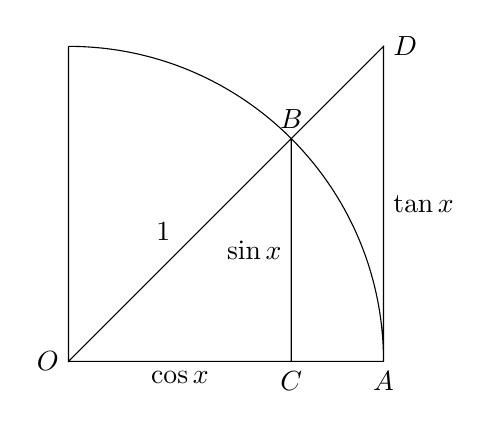
\begin{tikzpicture}
\pgfmathsetmacro{\r}{4}
\pgfmathsetmacro{\cx}{\r/sqrt(2)}
\coordinate (O) at (0,0);
\coordinate (A) at (\r,0);
\coordinate (B) at (\cx,\cx);
\coordinate (C) at (\cx,0);
\coordinate (D) at (\r,\r);
\draw (O)node[left]{\(O\)} -- (C)node[below]{\(C\)}node[midway,below]{\(\cos x\)} -- (A)node[below]{\(A\)}arc[start angle=0,end angle=90,radius=\r] (C) -- (B)node[above]{\(B\)}node[midway,left]{\(\sin x\)} -- (O)node[midway,above left]{\(1\)} -- (0,\r) (B) -- (D)node[right]{\(D\)} -- (A)node[midway,right]{\(\tan x\)};
\end{tikzpicture}
\end{center}
由于在\(0 < x < \pi/2\)时,\[
0 < \sin x < x < \tan x
\implies
1 < \frac{x}{\sin x} < \frac{1}{\cos x}
\implies
\cos x < \frac{\sin x}{x} < 1.
\]
因为\(\lim\limits_{x\to0}\cos x = 1\),所以由\hyperref[theorem:极限.夹逼准则]{夹逼准则}可知,\(\lim\limits_{x\to0} \frac{\sin x}{x} = 1\).
\end{proof}
\end{example}

\begin{example}
\def\l{\lim\limits_{x\to0}}
求:\(\l \frac{\tan x}{x}\).
\begin{solution}
\(
\l \frac{\tan x}{x}
= \l \left(\frac{\sin x}{x} \cdot \frac{1}{\cos x}\right)
= \l \frac{\sin x}{x} \cdot \lim\limits_{x\to0}\frac{1}{\cos x}
= 1.
\)
\end{solution}
\end{example}

\begin{example}
\def\l{\lim\limits_{x\to0}}
求:\(\l \frac{1 - \cos x}{x^2}\).
\begin{solution}
\(
\l \frac{1 - \cos x}{x^2}
= \l \frac{2 \sin^2\frac{x}{2}}{x^2}
= \frac{1}{2} \l \frac{\sin^2\frac{x}{2}}{\left(\frac{x}{2}\right)^2}
= \frac{1}{2} \left(\l \frac{\sin \frac{x}{2}}{\frac{x}{2}}\right)^2
= \frac{1}{2}.
\)
\end{solution}
\end{example}

\begin{example}
求:\(\lim\limits_{x\to0}\frac{\arcsin x}{x}\).
\begin{solution}
令\(t = \arcsin x\),则\(x = \sin t\).当\(x\to0\)时,有\(t\to0\).于是由复合函数的极限运算法则得\[
\lim\limits_{x\to0}\frac{\arcsin x}{x}
= \lim\limits_{t\to0}\frac{t}{\sin t}
= 1.
\]
\end{solution}
\end{example}

\begin{example}
\def\l{\lim\limits_{x\to0}}
计算\(\l \frac{\sin \omega x}{x}\).
\begin{solution}
当\(\omega=0\)时,\[
\l \frac{\sin \omega x}{x} = \l 0 = 0;
\]当\(\omega\neq0\)时,\[
\l \frac{\sin \omega x}{x}
= \omega \cdot \l \frac{\sin \omega x}{\omega x}
= \omega.
\]综上,\(\l \frac{\sin \omega x}{x} = \omega\).
\end{solution}
\end{example}

\begin{example}
\def\l{\lim\limits_{x\to0}}
计算\(\l \frac{\sin mx}{\sin nx}\).
\begin{solution}
\(
\l \frac{\sin mx}{\sin nx}
= \frac{m}{n} \cdot \l \left( \frac{\sin mx}{mx} \cdot \frac{nx}{\sin nx} \right)
= \frac{m}{n}
\).
\end{solution}
\end{example}

\begin{example}
\def\l#1{\lim\limits_{#1}}
计算\(\l{x\to\pi} \frac{\sin mx}{\sin nx} \quad(m,n\in\mathbb{Z})\).
\begin{solution}
\begin{align*}
\l{x\to\pi} \frac{\sin mx}{\sin nx}
&\xlongequal{t=x-\pi}
\l{t\to0} \frac{\sin m(t+\pi)}{\sin n(t+\pi)}
= \l{t\to0} \frac{(-1)^m}{(-1)^n} \frac{\sin mt}{\sin nt} \\
&= \l{t\to0} \frac{(-1)^m}{(-1)^n} \frac{\sin mt}{mt} \frac{m}{n} \frac{nt}{\sin nt}
= (-1)^{m-n} \frac{m}{n}.
\end{align*}
\end{solution}
\end{example}

\begin{example}
求:\(\lim\limits_{n\to\infty}\frac{1 \cdot 3 \cdot 5 \dotsm (2n-1)}{2 \cdot 4 \cdot 6 \dotsm (2n)}\).
\begin{solution}
因为\((2n)^2 = 4n^2 > 4n^2-1 = (2n-1)(2n+1)\),\(2n > \sqrt{(2n-1)(2n+1)}\),所以\[
2 > \sqrt{1 \cdot 3},
4 > \sqrt{3 \cdot 5},
6 > \sqrt{5 \cdot 7},
\dotsc,
\]故\[
\frac{1 \cdot 3 \cdot 5 \dotsm (2n-1)}{2 \cdot 4 \cdot 6 \dotsm (2n)}
< \frac{1 \cdot 3 \cdot 5 \dotsm (2n-1)}{\sqrt{1 \cdot 3} \sqrt{3 \cdot 5} \sqrt{5 \cdot 7} \dotsm \sqrt{(2n-1)(2n+1)}}
= \frac{1}{\sqrt{2n+1}}.
\]

因为\(0 < \frac{1 \cdot 3 \cdot 5 \dotsm (2n-1)}{2 \cdot 4 \cdot 6 \dotsm (2n)} < \frac{1}{\sqrt{2n+1}}\),而\[
\lim\limits_{n\to\infty}0 = \lim\limits_{n\to\infty}\frac{1}{\sqrt{2n+1}} = 0,
\]所以\(\lim\limits_{n\to\infty}\frac{1 \cdot 3 \cdot 5 \dotsm (2n-1)}{2 \cdot 4 \cdot 6 \dotsm (2n)} = 0\).
\end{solution}
\end{example}

\begin{example}
\renewcommand\l[1][]{\lim\limits_{x\to0\ifx\relax#1\relax\else^{#1}\fi}}
证明:\(\l \sqrt[n]{1+x} = 1\).
\begin{proof}
当\(x > 0\)时,因为\(1 < \sqrt[n]{1+x} < 1+x\),且\(\l[+] 1 = \l[+](1+x) = 1\),所以\[
\l[+] \sqrt[n]{1+x} = 1;
\]

当\(-1 < x < 0\)时,因为\(1+x < \sqrt[n]{1+x} < 1\),且\(\l[-] 1 = \l[+-](1+x) = 1\),所以\[
\l[-] \sqrt[n]{1+x} = 1.
\]

综上,\[
\l \sqrt[n]{1+x} = 1.
\qedhere
\]
\end{proof}
\end{example}

\begin{example}
证明:\(\lim\limits_{x\to0^+} x \floor*{\frac{1}{x}} = 1\).
\begin{proof}
令\(t=1/x\),那么\[
x \floor*{\frac{1}{x}} = \frac{1}{t} \floor{t}.
\]又因为\[
t - 1 < \floor{t} \leqslant t,
\]\[
1 - \frac{1}{t} < \frac{1}{t} \floor{t} \leqslant 1;
\]而\[
\lim\limits_{t\to+\infty} 1 - \frac{1}{t} = 1,
\quad
\lim\limits_{t\to+\infty} 1 = 1,
\]所以\[
\lim\limits_{x\to0^+} x \floor*{\frac{1}{x}} = \lim\limits_{t\to+\infty} \frac{1}{t} \floor{t} = 1.
\qedhere
\]
\end{proof}
\end{example}

\subsection{单调有界定理}
\begin{theorem}\label{theorem:极限.数列的单调有界定理}
单调有界数列必有极限.
\begin{proof}
不妨设数列\(\{a_n\}\)是单调增加的,即\[
	a_n \leqslant a_{n+1},
	\quad n=1,2,\dotsc;
	\eqno(1)
\]
又设\(\{a_n\}\)有界,且\[
	\abs{a_n} < c,
	\quad n=1,2,\dotsc.
	\eqno(2)
\]

现在我们把连续统分成两个集合\(A\)和\(B\),
把大于所有\(a_n\)的任何实数(例如数\(c\))放入集合\(B\),
而把其余的所有实数放入\(A\),即取\[
	B = \Set{ x \in \mathbb{R} \given x > a_n\ (n=1,2,\dotsc) },
	\eqno(3)
\]\[
	A = \mathbb{R} - B.
	\eqno(4)
\]
显然\(\Set{A,B}\)是\(\mathbb{R}\)的一个分割.
设\(\alpha\)是这个分割的界限,
那么必有\[
	a_n \leqslant \alpha,
	\quad n=1,2,\dotsc;
	\eqno(5)
\]
这是因为假设这个数列的某一项\(a_m\)满足\(a_m > \alpha\),
依照界限的定义会有\(a_m \in B\),而这与\(B\)的定义式(3)矛盾.

假设“\(\alpha\)不是\(\{a_n\}\)的极限”,
根据数列发散的定义,\[
	\exists\varepsilon>0,
	\forall n\in\mathbb{N}^+,
	\exists n_0>n
	\bigl( \abs{a_{n_0} - \alpha} > \varepsilon \bigr)
\]成立;
由(5)可知,\(\abs{a_{n_0} - \alpha} = \alpha - a_{n_0}\);
又因为\(\{a_n\}\)是单调增加的,
所以\(a_{n_0} \geqslant a_n\),
\(-a_{n_0} \leqslant -a_n\),
\(\alpha - a_{n_0} \leqslant \alpha - a_n\).
因此,\(\exists\varepsilon>0\),对\(\forall n\in\mathbb{N}^+\),都有\[
	\alpha - a_n > \varepsilon
	\quad\text{或}\quad
	a_n < \alpha - \varepsilon.
	\eqno(6)
\]
结合集合\(B\)的定义(3),由(6)便得\(\alpha - \varepsilon \in B\);
但由\(\alpha - \varepsilon < \alpha\)可知,应该有\((\alpha - \varepsilon) \in A\);
矛盾!因此假设不成立,\(\alpha\)就是数列\(\{a_n\}\)的极限,
即\(\lim\limits_{n\to\infty} a_n = \alpha\).
\end{proof}
\end{theorem}

由\cref{theorem:极限.收敛数列的有界性} 可知,收敛的数列一定有界.
但是,我们也知道,有界的数列不一定收敛,例如\[
	\{ x_n = \sin n \}, \qquad
	\{ y_n = (-1)^n \}.
\]
现在\cref{theorem:极限.数列的单调有界定理} 表明:
如果数列不仅有界,而且是单调的,那么这数列的极限必定存在,也就是这数列一定收敛.

相应于单调有界数列必有极限的准则,函数极限也有类似的准则.
\begin{theorem}\label{theorem:极限.函数的单调有界定理}
设函数\(f(x)\)在点\(x_0\)的某个左邻域\((x_0-\delta,x_0)\)内单调并且有界,则\(f(x)\)在\(x_0\)的左极限\(f(x_0^-)\)必定存在.
\end{theorem}

\begin{example}[重要极限II]
试证:极限\(\lim\limits_{x \to \infty}\left(1 + \frac{1}{x}\right)^x\)存在.
\begin{proof}
考虑\(x\)取正整数\(n\)而趋于\(+\infty\)的情形.设\(x_n=\left(1+\frac{1}{n}\right)^n\),根据牛顿二项公式,有\begin{align*}
x_n &= \left(1+\frac{1}{n}\right)^n
= \sum\limits_{k=0}^n \frac{n!}{k! (n-k)!} \frac{1}{n^k} \\
&= 1 + \frac{n}{1!}\frac{1}{n} + \frac{n(n-1)}{2!}\frac{1}{n^2} + \frac{n(n-1)(n-2)}{3!}\frac{1}{n^3} + \dotsb \\
&\qquad+ \frac{n(n-1)\dotsm(n-n+1)}{n!}\frac{1}{n^n} \\
&= 1 + 1 + \frac{1}{2!}\left(1-\frac{1}{n}\right) + \frac{1}{3!}\left(1-\frac{1}{n}\right)\left(1-\frac{2}{n}\right) + \dotsb \\
&\qquad+ \frac{1}{n!}\left(1-\frac{1}{n}\right)\left(1-\frac{2}{n}\right)\dotsm\left(1-\frac{n-1}{n}\right),
\end{align*}
类似地,\begin{align*}
x_{n+1}
&= 1 + 1 + \frac{1}{2!}\left(1-\frac{1}{n+1}\right) + \frac{1}{3!}\left(1-\frac{1}{n+1}\right)\left(1-\frac{2}{n+1}\right) + \dotsb \\
&\qquad+ \frac{1}{n!}\left(1-\frac{1}{n+1}\right)\left(1-\frac{2}{n+1}\right)\dotsm\left(1-\frac{n-1}{n+1}\right) \\
&\qquad+ \frac{1}{(n+1)!}\left(1-\frac{1}{n+1}\right)\left(1-\frac{2}{n+1}\right)\dotsm\left(1-\frac{n}{n+1}\right),
\end{align*}
比较\(x_n\)和\(x_{n+1}\)的展开式,可以看到除前两项外,\(x_n\)的每一项都小于\(x_{n+1}\)的对应项,并且\(x_{n+1}\)还多了最后一项\[
\frac{1}{(n+1)!}\left(1-\frac{1}{n+1}\right)\left(1-\frac{2}{n+1}\right)\dotsm\left(1-\frac{n}{n+1}\right) > 0,
\]因此\[
x_n < x_{n+1},
\]这就说明数列\(\{x_n\}\)是单调增加的.

又因为\[
x_n < 1 + 1 + \frac{1}{2!} + \frac{1}{3!} + \dotsb + \frac{1}{n!}
< 1 + 1 + \frac{1}{2} + \frac{1}{2^2} + \dotsb + \frac{1}{2^{n-1}}
= 3 - \frac{1}{2^{n-1}} < 3,
\]这就说明数列\(\{x_n\}\)是有界的.

既然数列\(\{x_n\}\)是单调增加的,%
又是有界的,%
那么数列\(\{x_n\}\)的极限一定存在,%
记它的极限值为常数\(e\).

再设\(n \leqslant x < n+1\),则\[
\left(1+\frac{1}{n+1}\right)^n < \left(1+\frac{1}{x}\right)^x < \left(1+\frac{1}{n}\right)^{n+1},
\]且当\(n\to\infty\)时,\(x\to\infty\),而\[
\lim\limits_{n\to\infty}\left(1+\frac{1}{n+1}\right)^n
=\lim\limits_{n\to\infty}\frac{\left(1+\frac{1}{n+1}\right)^{n+1}}{1+\frac{1}{n+1}} = e,
\]\[
\lim\limits_{n\to\infty}\left(1+\frac{1}{n}\right)^{n+1}
=\lim\limits_{n\to\infty}\left[\left(1+\frac{1}{n}\right)^n\cdot\left(1+\frac{1}{n}\right)\right]=e,
\]应用\hyperref[theorem:极限.夹逼准则]{夹逼准则}可得\[
\lim\limits_{x\to+\infty}\left(1+\frac{1}{x}\right)^x = e.
\]令\(x=-(t+1)\),则\(x\to-\infty\)时,\(t\to+\infty\),从而\begin{align*}
\lim\limits_{x\to-\infty}\left(1+\frac{1}{x}\right)^x
&=\lim\limits_{t\to+\infty}\left(1-\frac{1}{t+1}\right)^{-(t+1)}
=\lim\limits_{t\to+\infty}\left(\frac{t}{t+1}\right)^{-(t+1)} \\
&=\lim\limits_{t\to+\infty}\left(1+\frac{1}{t}\right)^{t+1}
=\lim\limits_{t\to+\infty}\left[\left(1+\frac{1}{t}\right)^t\cdot\left(1+\frac{1}{t}\right)\right]=e.
\end{align*}

综上所述,由于\[
\lim\limits_{x\to+\infty}\left(1+\frac{1}{x}\right)^x
= \lim\limits_{x\to-\infty}\left(1+\frac{1}{x}\right)^x
= e,
\]所以\begin{equation}\label{equation:极限.重要极限II}
\lim\limits_{x\to\infty} \left(1+\frac{1}{x}\right)^x = e.
\end{equation}
这就说明函数极限\(\lim\limits_{x\to\infty} \left(1+\frac{1}{x}\right)^x\)存在.
\end{proof}
\end{example}
我们称上面所说的常数\(e\)为“\textbf{欧拉常数} \(e\)”.

另外,利用复合函数的极限运算法则,可得
\begin{equation}
\lim\limits_{z\to0}(1+z)^{\frac{1}{z}}
\xlongequal{z=1/x}
\lim\limits_{x\to\infty}\left(1+\frac{1}{x}\right)^x
= e.
\end{equation}

\begin{figure}[ht]
\centering
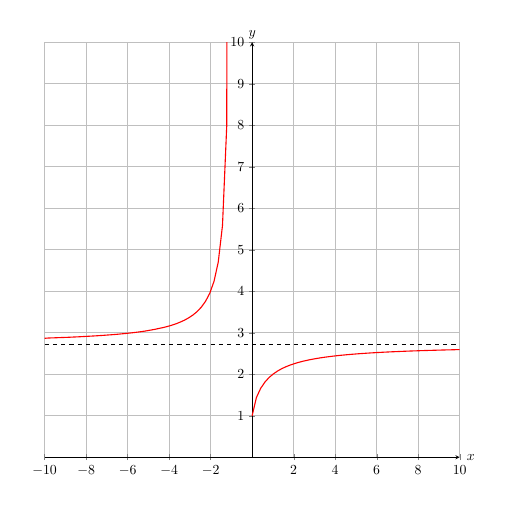
\begin{tikzpicture}[scale=.5]
% Mathematica: Plot[{E, (1 + 1/x)^x}, {x, -10, 10}, PlotRange -> {0, 10}, AspectRatio -> Automatic, PlotStyle -> {{Dashed, Thin}, Thin}]
\begin{axis}[
xmin=-10,xmax=10,ymin=0,ymax=10,grid=both,width=\textwidth,height=\textwidth,
xlabel={\(x\)},
ylabel={\(y\)},
enlarge x limits=0.1,
enlarge y limits=0.1,
axis lines = middle,
x label style={at={(ticklabel* cs:1.00)}, inner sep=5pt, anchor=west},
y label style={at={(ticklabel* cs:1.00)}, inner sep=2pt, anchor=south},
]
\addplot[domain=-10:-0,samples=50,thick,red]{(1+1/x)^x};
\addplot[domain=+0:+10,samples=50,thick,red]{(1+1/x)^x};
\addplot[dashed,domain=-10:10]{e};
\end{axis}
\end{tikzpicture}
\caption{函数\(y=\left(1+\tfrac{1}{x}\right)^x\)的图像}
\label{figure:极限.函数(1+1/x)^x的图像}
\end{figure}

如\cref{figure:极限.函数(1+1/x)^x的图像} 所示,%
我们可以画出函数\(y=\left(1+\frac{1}{x}\right)^x\ (x<-1 \lor x>0)\)的图像.
可见,直线\(y=e\)是函数\(y=\left(1+\frac{1}{x}\right)^x\)的图像的水平渐近线.
另外,易证\[
\lim\limits_{x\to0^+} \left(1+\frac{1}{x}\right)^x = 1,
\qquad
\lim\limits_{x\to1^-} \left(1+\frac{1}{x}\right)^x = +\infty.
\]


\begin{example}
求:\(\lim\limits_{x \to \infty}\left(1 - \frac{1}{x}\right)^x\).
\begin{solution}
令\(t = -x\),则当\(x \to +\infty\)时,\(t \to -\infty\),于是\[
\lim\limits_{x \to +\infty}\left(1 - \frac{1}{x}\right)^x
= \lim\limits_{t \to -\infty}\left(1 + \frac{1}{t}\right)^{-t}
= \lim\limits_{t \to -\infty}\frac{1}{\left(1 + \frac{1}{t}\right)^t}
= \frac{1}{e}.
\]
\end{solution}

画出函数\(y=\left(1-\frac{1}{x}\right)^x\ (x<0 \lor x\geqslant1)\)的图像如\cref{figure:极限.函数(1-1/x)^x的图像}.
\begin{figure}[ht]
\centering
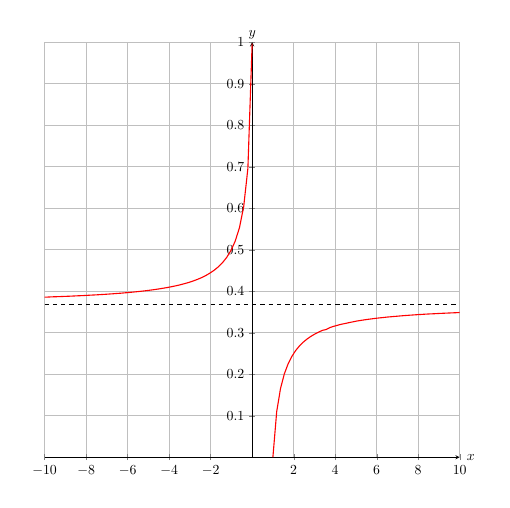
\begin{tikzpicture}[scale=.5]
% Mathematica: Plot[{1/E, (1 - 1/x)^x}, {x, -10, 10}, PlotRange -> {0, 1}, PlotStyle -> {{Dashed, Thin}, Thin}]
\begin{axis}[
xmin=-10,xmax=10,ymin=0,ymax=1,grid=both,width=\textwidth,height=\textwidth,
xlabel={\(x\)},
ylabel={\(y\)},
enlarge x limits=1,
enlarge y limits=1,
axis lines = middle,
x label style={at={(ticklabel* cs:1.00)}, inner sep=5pt, anchor=west},
y label style={at={(ticklabel* cs:1.00)}, inner sep=2pt, anchor=south},
]
\addplot[domain=-10:-0,samples=50,thick,red]{(1-1/x)^x};
\addplot[dashed,domain=-10:10]{1/e};
\addplot[domain=+1:+10,samples=50,thick,red]{(1-1/x)^x};
\end{axis}
\end{tikzpicture}
\caption{函数\(y=\left(1-\tfrac{1}{x}\right)^x\)的图像}
\label{figure:极限.函数(1-1/x)^x的图像}
\end{figure}
可见,直线\(y=\frac{1}{e}\)是函数\(y=\left(1-\frac{1}{x}\right)^x\)的图像的水平渐近线.
另外,易证\[
\lim\limits_{x\to0^-} \left(1-\frac{1}{x}\right)^x = 1.
\]
\end{example}

\subsection{柯西极限存在准则}
\begin{theorem}[柯西极限存在准则]\label{theorem:极限.数列的柯西极限存在准则}
数列\(\{x_n\}\)收敛的充分必要条件是:
对于任意给定的正数\(\varepsilon\),
存在着这样的正整数\(N\),
使得当\(m>N\)且\(n>N\)时,就有\[
	\abs{x_n-x_m}<\varepsilon.
\]
\begin{proof}
必要性.
设\(\lim\limits_{n\to\infty}x_n = a\).
由数列极限的定义,
对于\(\forall\varepsilon>0\),
\(\exists N \in \mathbb{N}^+\),
当\(n > N\)时,有\[
	\abs{x_n - a} < \frac{\varepsilon}{2};
\]
同样地,当\(m > N\)时,有\[
	\abs{x_m - a} < \frac{\varepsilon}{2}.
\]
因此,当\(n > N\)且\(m > N\)时,有\[
	\abs{x_n - x_m} = \abs{(x_n - a) - (x_m - a)}
	\leqslant \abs{x_n - a} + \abs{x_m - a}
	< \frac{\varepsilon}{2} + \frac{\varepsilon}{2}
	= \varepsilon.
	\qedhere
\]
%TODO 未证充分性
\end{proof}
\end{theorem}
柯西极限存在准则有时也叫作\emph{柯西审敛原理}.

它可以用“\(\varepsilon-\delta\)”语言表示如下.
数列\(\{x_n\}\)收敛的充分必要条件是:\[
\forall\varepsilon>0,
\exists N\in\mathbb{N}^+,
\forall n,m \geqslant N
\bigl(
	\abs{x_n-x_m}<\varepsilon
\bigr)
\]或\[
\forall\varepsilon>0,
\exists N\in\mathbb{N}^+
\bigl[
	n>N
	\implies
	\forall p\in\mathbb{N}^+
	\bigl(
		\abs{x_{n+1} + x_{n+2} + \dotsb + x_{n+p}} < \varepsilon
	\bigr)
\bigr].
\]

那么它的逆否命题可以表达如下.
数列\(\{x_n\}\)发散的充分必要条件是:\[
\exists\varepsilon_0>0,\forall N\in\mathbb{N}^+ \bigl[
	n > N
	\land
	\exists p\in\mathbb{N}^+ \bigl(
		\abs{x_{n+1} + x_{n+2} + \dotsb + x_{n+p}} \geqslant \varepsilon_0
	\bigr)
\bigr].
\]

类似地,函数极限也有自己的柯西审敛原理.
\begin{theorem}\label{theorem:极限.函数的柯西极限存在准则}
函数\(f(x)\)在点\(a\)的极限存在的充要条件是:对于任意给定的正数\(\varepsilon\),存在正数\(\delta\),使得当\(0 < \abs{x_1 - a} < \delta\)且\(0 < \abs{x_2 - a} < \delta\)时,就有\(\abs{f(x_1) - f(x_2)} < \varepsilon\).
\end{theorem}

\section{欧拉常数\texorpdfstring{\(e\)}{e}}
可以证明,欧拉常数\(e\)是一个无理数,也是一个超越数,它的近似值约为2.718.

我们在前一节利用单调有界定理证明了数列极限\[
\lim\limits_{n\to\infty} \left(1+\frac{1}{n}\right)^n = e,
\]
那么,当\(x\neq0\)时,有
\begin{align*}
\lim\limits_{n\to\infty} \left(1+\frac{x}{n}\right)^n
&= \lim\limits_{n\to\infty} \left(1+\frac{1}{n/x}\right)^{\frac{n}{x} \cdot x} \\
&\xlongequal{t=n/x} \left[ \lim\limits_{t\to\infty} \left(1+\frac{1}{t}\right)^t \right]^x
= e^x;
\end{align*}
当\(x=0\)时,有\[
\lim\limits_{n\to\infty} \left(1+\frac{x}{n}\right)^n
= \lim\limits_{n\to\infty} (1+0)^n
= \lim\limits_{n\to\infty} 1
= 1 \equiv e^0;
\]
因此我们可以定义“以\(e\)为底数的指数函数”为
\begin{equation}\label{equation:特殊函数.以e为底数的指数函数的极限定义}
e^x
\defeq
\lim\limits_{n\to\infty} \left(1+\frac{x}{n}\right)^n.
\end{equation}

我们还可以定义“以\(e\)为底数的对数函数”为
\begin{equation}\label{equation:特殊函数.以e为底数的对数函数的极限定义}
\ln x
\defeq
\lim\limits_{n\to\infty} n \left( \sqrt[n]{x} - 1 \right).
\end{equation}

\section{无穷小的比较}
\subsection{无穷小的比较方法}
\begin{definition}
\newcommand{\lf}[1][]{\lim \frac{\beta}{\alpha^{#1}}}
设\(\alpha\)和\(\beta\)都是在同一个自变量的变化过程中的无穷小,且\(\alpha\neq0\).
\begin{enumerate}
\item 如果\(\lf=0\),就说\(\beta\)是比\(\alpha\)\textbf{高阶}的无穷小,记作\(\beta=o(\alpha)\);
\item 如果\(\lf=\infty\),就说\(\beta\)是比\(\alpha\)\textbf{低阶}的无穷小.
\item 如果\(\lf=c\neq0\),就说\(\beta\)是比\(\alpha\)\textbf{同阶}无穷小;
\item 如果\(\lf[k]=c\neq0\),\(k>0\),就说\(\beta\)是关于\(\alpha\)的\(k\)\textbf{阶}无穷小.
\item 如果\(\lf=1\),就说\(\beta\)与\(\alpha\)是\textbf{等价无穷小},记作\(\alpha\sim\beta\).
\end{enumerate}
\end{definition}
显然,等价无穷小是同阶无穷小的特殊情形,即\(c=1\)的情形.

应该注意到,记号\(o(\alpha)\)实际上是由所有满足\[
\lim \frac{\beta}{\alpha} = 0
\]的函数\(\beta\)构成的集合,即\[
o(\alpha) = \Set*{ \beta \given \lim \frac{\beta}{\alpha} = 0 }.
\]虽然在给定\(\lim \frac{\beta}{\alpha}\)时,我们本该用记号\(\beta \in o(\alpha)\)表示\(\beta\)是比\(\alpha\)高阶的无穷小,但我们在后面很快就会看到使用记号\(\beta = o(\alpha)\)的诸多好处.

\begin{example}
因为\(\lim\limits_{x\to0} \frac{3x^2}{x} = 0\),所以当\(x\to0\)时,\(3x^2\)是比\(x\)高阶的无穷小,即\(3x^2 = o(x)\ (x\to0)\).

因为\(\lim\limits_{n\to\infty} \frac{1/n}{1/n^2} = \infty\),所以当\(n\to\infty\)时,\(\frac{1}{n}\)是比\(\frac{1}{n^2}\)低阶的无穷小.

因为\(\lim\limits_{x\to3} \frac{x^2-9}{x-3} = 6\),所以当\(x\to3\)时,\(x^2-9\)与\(x-3\)是同阶无穷小.

因为\(\lim\limits_{x\to0} \frac{1-\cos x}{x^2} = \frac{1}{2}\),所以当\(x\to0\)时,\(1-\cos x\)是关于\(x\)的二阶无穷小.

因为\(\lim\limits_{x\to0} \frac{\sin x}{x} = 1\),所以当\(x\to0\)时,\(\sin x\)与\(x\)是等价无穷小,即\(\sin x \sim x\ (x\to0)\).
\end{example}

\begin{example}
因为\[
\lim\limits_{n\to\infty} n^k \cdot o\left(\frac{1}{n^k}\right)
= \lim\limits_{n\to\infty} n^{k-l} \left[ n^l \cdot o\left(\frac{1}{n^k}\right) \right] = 0,
\]所以\begin{equation}
n^l \cdot o\left(\frac{1}{n^k}\right) = o\left(\frac{1}{n^{k-l}}\right) \quad(n\to\infty).
\end{equation}
\end{example}

\begin{example}
\def\l{\lim\limits_{n\to\infty}}
考虑到\[
\l \frac{o(n^2) + o(n^3)}{n^3}
= \l \frac{1}{n}\cdot\frac{o(n^2)}{n^2} + \l \frac{o(n^3)}{n^3}
= 0 + 0 = 0,
\]可以推断\[
q > p \implies o(n^p) + o(n^q) = o(n^q)\ (n\to\infty).
\]

考虑到\[
\l \frac{o(n^2) \cdot o(n^3)}{n^5}
= \l \frac{o(n^2)}{n^2}\cdot\frac{o(n^3)}{n^3}
= 0,
\]可以推断\begin{equation}
o(n^p) \cdot o(n^q) = o(n^{p+q}).
\end{equation}
\end{example}

\begin{example}
证明:当\(x\to0\)时,\(\sqrt[n]{1+x} - 1 \sim \frac{1}{n} x\).
\begin{proof}
因为\begin{align*}
\frac{\sqrt[n]{1+x} - 1}{\frac{1}{n} x}
&= \frac{(\sqrt[n]{1+x})^n - 1}{\frac{1}{n} x \left[ \sqrt[n]{(1+x)^{n-1}} + \sqrt[n]{(1+x)^{n-2}} + \dotsb + 1 \right]} \\
&= \frac{n}{\sqrt[n]{(1+x)^{n-1}} + \sqrt[n]{(1+x)^{n-2}} + \dotsb + 1},
\end{align*}
而\[
\lim\limits_{x\to0} \sqrt[n]{(1+x)^m} = 1,
\]所以\[
\lim\limits_{x\to0} \frac{\sqrt[n]{1+x} - 1}{\frac{1}{n} x} = \lim\limits_{x\to0} \frac{n}{1 \cdot n} = 1,
\]也就是说\(\sqrt[n]{1+x} - 1 \sim \frac{1}{n} x \quad(x\to0)\).
\end{proof}
\end{example}

\begin{theorem}\label{theorem:极限.无穷小的比较1}
\(\beta\)与\(\alpha\)是等价无穷小的充分必要条件为\[\beta=\alpha+o(\alpha).\]
\begin{proof}
必要性.设\(\alpha\sim\beta\),则\[
\lim\frac{\beta-\alpha}{\alpha}
=\lim\left(\frac{\beta}{\alpha}-1\right)
=\lim\frac{\beta}{\alpha}-1 = 0,
\]因此\(\beta-\alpha=o(\alpha)\),即\(\beta=\alpha+o(\alpha)\).

充分性.设\(\beta=\alpha+o(\alpha)\),则\[
\lim\frac{\beta}{\alpha}
=\lim\frac{\alpha+o(\alpha)}{\alpha}
=\lim\left(1+\frac{o(\alpha)}{\alpha}\right) = 1,
\]因此\(\alpha\sim\beta\).
\end{proof}
\end{theorem}

\begin{theorem}\label{theorem:极限.无穷小的比较2}
设\(\alpha\sim\alpha'\),\(\beta\sim\beta'\),且\(\lim\frac{\beta'}{\alpha'}\)存在,则\[
\lim\frac{\beta}{\alpha}=\lim\frac{\beta'}{\alpha'}.
\]
\begin{proof}
由\(\alpha\sim\alpha'\)和\(\beta\sim\beta'\)有\(\lim\frac{\alpha'}{\alpha} = 1\),\(\lim\frac{\beta}{\beta'} = 1\),因此\[
\lim\frac{\beta}{\alpha}
= \lim \left( \frac{\beta}{\beta'} \cdot \frac{\beta'}{\alpha'} \cdot \frac{\alpha'}{\alpha} \right)
= \lim\frac{\beta}{\beta'} \cdot \lim \frac{\beta'}{\alpha'} \cdot \lim\frac{\alpha'}{\alpha}
= 1 \cdot \lim \frac{\beta'}{\alpha'} \cdot 1
= \lim \frac{\beta'}{\alpha'}.
\qedhere
\]
\end{proof}
\end{theorem}

\begin{theorem}[和差取大规则]\label{theorem:极限.无穷小的比较3}
设\(\beta=o(\alpha)\),则\(\alpha\pm\beta\sim\alpha\).
\begin{proof}
显然有\[
\lim \frac{\alpha\pm\beta}{\alpha}
= \lim \frac{\alpha\pm o(\alpha)}{\alpha}
= \lim \frac{\alpha}{\alpha} \pm \lim \frac{o(\alpha)}{\alpha}
= 1 \pm 0 = 1.
\qedhere
\]
\end{proof}
\end{theorem}

\begin{theorem}[和差代替规则]\label{theorem:极限.无穷小的比较4}
设\(\alpha\sim\alpha'\),\(\beta\sim\beta'\),\(\beta\)与\(\alpha\)不是等价无穷小,则\[
\alpha\pm\beta\sim\alpha'\pm\beta',
\qquad
\lim \frac{\alpha\pm\beta}{\gamma} = \lim \frac{\alpha'\pm\beta'}{\gamma}.
\]
\begin{proof}
既然\(\alpha\)与\(\beta\)不是等价无穷小,不妨设\(\beta\)是比\(\alpha\)高阶的无穷小,即\(\beta = o(\alpha)\),那么由\hyperref[theorem:极限.无穷小的比较3]{和差取大规则}有\(\alpha\pm\beta \sim \alpha\).
又由\cref{theorem:极限.无穷小的比较2} 可知\[
\lim \frac{\alpha'\pm\beta'}{\alpha'}
= 1 \pm \lim \frac{\beta'}{\alpha'}
= 1 \pm \lim \frac{\beta}{\alpha}
= \lim \frac{\alpha\pm\beta}{\alpha}
= 1,
\]即\(\alpha'\pm\beta' \sim \alpha'\).
那么由等价无穷小关系的传递性,可知\(\alpha\pm\beta \sim \alpha'\pm\beta'\).
\end{proof}
\end{theorem}

\begin{theorem}[因式代替规则]\label{theorem:极限.无穷小的比较5}
设\(\alpha\sim\beta\),且函数\(\varphi\)有界或\(\lim\varphi\)存在,则\[
\lim \alpha \varphi = \lim \beta \varphi,
\quad\text{即}\quad
\alpha \varphi \sim \beta \varphi.
\]
\end{theorem}
这里其实说明无穷小与有界函数之积也是无穷小.

\begin{property}\label{theorem:极限.无穷小的比较6}
无穷小的等价关系具有以下性质:
\begin{enumerate}
\item {\bf 自反性},即\(\alpha \sim \alpha\);
\item {\bf 对称性},即\(\alpha \sim \beta \implies \beta \sim \alpha\);
\item {\bf 传递性},即\(\alpha \sim \beta, \beta \sim \gamma \implies \alpha \sim \gamma\).
\end{enumerate}
\end{property}

\subsection{常见的等价无穷小}
常见的等价无穷小有:
\begin{enumerate}
\item \(\sin x \sim \tan x \sim \arcsin x \sim \arctan x \sim \ln(1+x) \sim e^x-1 \sim x\ (x\to0)\);
\item \(\sqrt[n]{1+x} - 1 \sim \frac{1}{n} x\ (x\to0)\);
\item \(\forall a\in\mathbb{R}^*: (1+x)^a-1 \sim ax\ (x\to0)\);
\item \(1 - \cos x \sim \frac{1}{2} x^2\ (x\to0)\);
\item \(a^x - 1 \sim x \ln a\ (x\to0)\).
\end{enumerate}

\begin{example}
证明:若函数\(\alpha,\beta\)满足\(\lim \alpha\beta = 0\)且\(\lim \beta = 0\),则\[
(1+\beta)^{\alpha} - 1 \sim \alpha\beta \quad(\beta\to0).
\]
\begin{proof}
因为\(\ln(1+\beta) \sim \beta\ (\beta\to0)\),所以\[
(1+\beta)^{\alpha} - 1
= e^{\alpha \ln(1+\beta)} - 1
\sim e^{\alpha\beta} - 1
\sim \alpha\beta
\quad(\beta\to0).
\qedhere
\]
\end{proof}
\end{example}

\section{施托尔茨定理}

\begin{theorem}[施托尔茨定理I]\label{theorem:极限.施托尔茨定理1}
设数列\(\{x_n\}\)、\(\{y_n\}\).
若\(y_n < y_{n+1}\ (n=1,2,\dotsc)\),且\(y_n \to +\infty\ (n\to\infty)\),且\[
\lim\limits_{n\to\infty} \frac{x_{n+1}-x_n}{y_{n+1}-y_n} = C\in[-\infty,+\infty],
\]那么有\[
\lim\limits_{n\to\infty} \frac{x_n}{y_n}
= \lim\limits_{n\to\infty} \frac{x_{n+1}-x_n}{y_{n+1}-y_n}
= C.
\]
\begin{proof}%TODO
设\(\lim\limits_{n\to\infty} \frac{x_{n+1}-x_n}{y_{n+1}-y_n} = C\in(-\infty,+\infty)\),%
故对\(\forall\varepsilon>0\),\(\exists N>0\),当\(n > N\)时,有\[
\abs{\frac{x_{n+1}-x_n}{y_{n+1}-y_n} - C} < \varepsilon
\]成立,即\[
C - \varepsilon < \frac{x_{n+1}-x_n}{y_{n+1}-y_n} < C + \varepsilon;
\]
由于\[
\frac{
(x_{N+1}-x_N)
+ (x_{N+2}-x_{N+1})
+ \dotsb
+ (x_{n+1}-x_n)
}{
(y_{N+1}-y_N)
+ (y_{N+2}-y_{N+1})
+ \dotsb
+ (y_{n+1}-y_n)
}
= \frac{x_{n+1}-x_N}{y_{n+1}-y_N},
\]再根据\cref{example:不等式.不同浓度的溶液的混合},于是有\[
C - \varepsilon <
\frac{x_{n+1}-x_N}{y_{n+1}-y_N}
< C + \varepsilon;
\]进而有\[
\lim\limits_{n\to\infty} \frac{x_{n+1}-x_N}{y_{n+1}-y_N}
= \lim\limits_{n\to\infty} \frac{\frac{x_{n+1}}{y_{n+1}}-\frac{x_N}{y_{n+1}}}{1-\frac{y_N}{y_{n+1}}}
= C;
\]又因为\(\lim\limits_{n\to\infty} y_n = +\infty\),%
注意到\(x_N\)、\(y_N\)是不随\(n\)变化的常数,%
于是有\(\lim\limits_{n\to\infty} \frac{x_N}{y_{n+1}}
= \lim\limits_{n\to\infty} \frac{y_N}{y_{n+1}}
= 0\),从而有\(\lim\limits_{n\to\infty} \frac{x_{n+1}}{y_{n+1}} = C\).
\end{proof}
\end{theorem}

\begin{theorem}[施托尔茨定理II]\label{theorem:极限.施托尔茨定理2}
设数列\(\{x_n\}\)、\(\{y_n\}\).
若\(x_n\to0\ (n\to\infty)\),\(y_n > y_{n+1}\ (n=1,2,\dotsc)\),且\(y_n\to0\ (n\to\infty)\),且\[
\lim\limits_{n\to\infty} \frac{x_{n+1}-x_n}{y_{n+1}-y_n} = C\in[-\infty,+\infty],
\]那么有\[
\lim\limits_{n\to\infty} \frac{x_n}{y_n}
= \lim\limits_{n\to\infty} \frac{x_{n+1}-x_n}{y_{n+1}-y_n}
= C.
\]
\end{theorem}

施托尔茨定理实际上是离散形式的洛必达法则,它适用于\(\frac{0}{0}\)、\(\frac{\infty}{\infty}\)或\(\frac{*}{\infty}\)三种情形.


\section{函数的连续性与间断点}

\subsection{函数的连续性}
\begin{definition}
设变量\(u\)从它的一个初值\(u_1\)变到终值\(u_2\),终值与初值的差\(u_2 - u_1\)就叫做变量\(u\)的\textbf{增量},记作\(\increment u\),即\[
\increment u = u_2 - u_1.
\]
\end{definition}
在实数域中,增量\(\increment u\)既可以是正的,也可以是负的.当\(\increment u > 0\)时,变量\(u\)从初值变到终值时是增大的;当\(\increment u < 0\)时,变量\(u\)从初值变到终值时是减小的.

\begin{definition}\label{definition:极限.函数在一点的连续性}
设函数\(y=f(x)\)在点\(x_0\)的某一邻域内有定义.
如果\[
\lim\limits_{\increment x\to0} \increment y
=\lim\limits_{\increment x\to0} [f(x_0 + \increment x)-f(x_0)]
=0,
\]或者\[
\lim\limits_{x \to x_0} f(x) = f(x_0),
\]或者\[
\forall \varepsilon > 0,
\exists \delta > 0
( 0 < \abs{x - x_0} < \delta \implies \abs{f(x) - f(x_0)} < \varepsilon )
\]那么就称“函数\(f(x)\)在点\(x_0\)\textbf{连续}(the function \(f(x)\) is continuous at \(x_0\))”,%
称“点\(x_0\)是函数\(f(x)\)的\textbf{连续点}(point of continuity)”.

如果\(f(x)\)在点\(x_0\)的某一左邻域内有定义,极限\(f(x_0^-) = \lim\limits_{x \to x_0^-} f(x)\)存在,且\[
f(x_0^-) = f(x_0),
\]则称“函数\(f(x)\)在点\(x_0\)\textbf{左连续}(the function \(f(x)\) is left-continuous at \(x_0\))”.

如果\(f(x)\)在点\(x_0\)的某一右邻域内有定义,极限\(f(x_0^+) = \lim\limits_{x \to x_0^+} f(x)\)存在,且\[
f(x_0^+) = f(x_0),
\]则称“函数\(f(x)\)在点\(x_0\)\textbf{右连续}(the function \(f(x)\) is right-continuous at \(x_0\))”.
\end{definition}

\begin{definition}
如果函数\(f(x)\)在\(\forall x \in (a,b)\)处都连续,%
那么称“函数\(f(x)\)在开区间\((a,b)\)内连续”.

如果函数\(f(x)\)不仅在\(\forall x \in (a,b)\)处都连续,%
还在点\(a\)处右连续,且在\(b\)处左连续,%
那么称“函数\(f(x)\)在闭区间\([a,b]\)上连续”.
\end{definition}
类似地可以定义函数\(f(x)\)在半开半闭区间\((a,b]\)或\([a,b)\)内连续的概念.

\begin{definition}\label{definition:函数族.连续函数族}
由区间\(I\)上全部的连续函数组成的集合,称作\textbf{连续函数族}\footnote{%
也可将“函数族”称为“函数空间”.%
},记作\(C(I)\)\footnote{%
当\(I=(a,b)\)时,可改写为\(C(a,b)\),以此类推.%
}.
\end{definition}

\begin{example}
证明:\(f(x) = \sin x\)是在\((-\infty,+\infty)\)上的连续函数.
\begin{proof}
要证\(f(x) = \sin x\)是在\((-\infty,+\infty)\)上的连续函数,只需证\[
\lim\limits_{\increment x\to0} [\sin(x+\increment x) - \sin x] = 0,
\]又因为\(
\sin(x+\increment x) - \sin x
= 2 \cos\left(x+\frac{\increment x}{2}\right) \sin\frac{\increment x}{2}
\),其中\(2 \cos\left(x+\frac{\increment x}{2}\right)\)是有界函数,而\(\sin\frac{\increment x}{2}\)是\(\increment x\to0\)时的无穷小,那么\(\sin(x+\increment x) - \sin x\)是\(\increment x\to0\)时的无穷小.
\end{proof}
\end{example}

\begin{example}
证明:若\(f(x)\)在\((-\infty,+\infty)\)内连续,且\(\lim\limits_{x \to \infty}f(x)\)存在,则\(f(x)\)必在\((-\infty,+\infty)\)内有界.
\begin{proof}
因为\(\lim\limits_{x \to \infty} f(x)\)存在,那么由函数极限的局部有界性定理可知,\[
\exists M>0,\exists X>0 \bigl[
\abs{x} > X \implies \abs{f(x)} \leqslant M
\bigr],
\]也就是说\(f(x)\)在区间\((-\infty,-X)\cup(X,+\infty)\)上有界.

又因为\(f(x)\)在\((-\infty,+\infty)\)内连续,所以\(f(x)\)在\([-X,X]\)上连续,进而\(f(x)\)在\([-X,X]\)上有界.

综上所述,\(f(x)\)在\((-\infty,+\infty)\)上有界.
\end{proof}
\end{example}

\begin{example}
设\(f \in C(\mathbb{R})\),且\(\forall x,y\in\mathbb{R} : f(x+y) = f(x) + f(y)\).
证明:\[
\forall x\in\mathbb{R} : f(x) = f(1) x.
\]
\begin{proof}
\def\f#1#2{f\left(\frac{#1}{#2}\right)}
令\(x=y=0\),得\(f(0+0) = f(0) + f(0)\),移项,得\(f(0) = 0\).

当\(x = m/n \in \mathbb{Q}\)时.因为\[
f(1) = \f{1}{n} + \f{n-1}{n}
= 2 \f{1}{n} + \f{n-2}{n}
= \dotsb
= n \f{1}{n},
\]所以\(f(1/n) = f(1) / n\),进而\[
\begin{split}
\f{m}{n}
&= \f{1}{n} + \f{m-1}{n}
= 2 \f{1}{n} + \f{m-2}{n} \\
&= \dotsb
= m \f{1}{n} = \frac{m}{n} f(1).
\end{split}
\]

当\(x \in \mathbb{Q}^C\)时.用有理数列逼近无理数证明题设成立.
\end{proof}
\end{example}

\subsection{连续曲线}
\begin{definition}
设平面曲线\(L\)的参数方程为\[
\left\{ \begin{array}{l}
x = \varphi(t) \\
y = \psi(t) \\
\end{array} \right.,
\quad
t \in [\alpha,\beta].
\]如果\(\varphi(t)\)、\(\psi(t)\)在\([\alpha,\beta]\)上连续,则称曲线\(L\)为\textbf{连续曲线}.
点\(\opair{\varphi(\alpha),\psi(\alpha)}\)称为曲线的\textbf{起点},%
点\(\opair{\varphi(\beta),\psi(\beta)}\)称为曲线的\textbf{终点}.

如果存在\(t_1\)、\(t_2\)满足\(\alpha \leqslant t_1 < t_2 \leqslant \beta\)
且\((t_1-\alpha)^2+(t_2-\beta)^2 \neq 0\),使得对应的两点重合,%
即\(\opair{\varphi(t_1),\psi(t_1)}=\opair{\varphi(t_2),\psi(t_2)}\)成立,%
则称该点为曲线\(L\)的\textbf{重点}.

无重点的连续曲线称为\textbf{若尔当曲线}或\textbf{简单曲线}.

仅起点和终点重合(即\(\opair{\varphi(\alpha),\psi(\alpha)}=\opair{\varphi(\beta),\psi(\beta)}\))的简单曲线称作\textbf{若尔当闭曲线}或者\textbf{简单闭曲线}.
\end{definition}

\subsection{函数的间断点}
设函数\(f(x)\)在点\(x_0\)的某去心邻域内有定义.
在此前提下,如果函数\(f(x)\)有下列三种情形之一:
\begin{enumerate}
\item 在\(x=x_0\)没有定义;
\item 虽在\(x=x_0\)有定义,但\(\lim\limits_{x \to x_0} f(x)\)不存在;
\item 虽在\(x=x_0\)有定义,且\(\lim\limits_{x \to x_0} f(x)\)存在,但\(\lim\limits_{x \to x_0} f(x) \neq f(x_0)\),%
\end{enumerate}
则称“函数\(f(x)\)在点\(x_0\)不连续”,%
称“点\(x_0\)是函数\(f(x)\)的\textbf{不连续点}或\textbf{间断点}(discontinuity)”.

\begin{definition}
如果\(\lim\limits_{x \to x_0}f(x) = \infty\),则称点\(x_0\)为函数的\textbf{无穷间断点}.

如果\(f(x)\)在点\(x_0\)的某一邻域是有界的,但其左、右极限均不存在,则称点\(x_0\)为函数的\textbf{振荡间断点}.

如果\(f(x)\)在点\(x_0\)没有定义,\(\lim\limits_{x \to x_0}f(x) = A\),则称点\(x_0\)为函数的\textbf{可去间断点}(removable discontinuity).

如果\(f(x)\)在点\(x_0\)的左、右极限存在但不相等,即\(\lim\limits_{x \to x_0^-}f(x) \neq \lim\limits_{x \to x_0^+}f(x)\),则称点\(x_0\)为函数的\textbf{跳跃间断点}(jump discontinuity).

如果\(x_0\)是函数\(f(x)\)的间断点,但左极限\(f(x_0^-)\)及右极限\(f(x_0^+)\)都存在,那么\(x_0\)称为函数\(f(x)\)的\textbf{第一类间断点}(discontinuity of the first kind).
不是第一类间断点的间断点,称为\textbf{第二类间断点}(discontinuity of the second kind).
\end{definition}
显然,可去间断点、跳跃间断点是第一类间断点,无穷间断点、振荡间断点是第二类间断点.

\begin{example}\label{example:极限.狄利克雷函数在实数域上处处不连续}
证明:狄利克雷函数\[
D(x) = \left\{ \begin{array}{ll}
1, & x \in \mathbb{Q}, \\
0, & x \in \mathbb{R} - \mathbb{Q}.
\end{array} \right.
\]在\(\mathbb{R}\)上处处不连续.
\begin{proof}
\(\forall x_0 \in \mathbb{R}\),一定存在全由有理数组成的数列\(\{s_n\}\)和全由无理数组成的数列\(\{t_n\}\)趋于点\(x_0\),这样就有\[
\lim\limits_{n\to\infty} D(s_n) = 1,
\qquad
\lim\limits_{n\to\infty} D(t_n) = 0.
\]
根据\hyperref[theorem:极限.海涅定理]{海涅定理}可知,\(\lim\limits_{x \to x_0} D(x)\)不存在.
\end{proof}
\end{example}

\begin{example}
证明:函数\(f(x) = x D(x)\)除在点\(x = 0\)处连续之外,在\(\mathbb{R}\)上其余各点均不连续.
\begin{proof}
先证\(f\)在点\(x = 0\)处连续.此时\(f(0) = 0\).
\(\forall \varepsilon > 0\),取\(\delta = \varepsilon\),当\(\abs{x - 0} = \abs{x} < \delta\)时,有\[
\abs{f(x) - f(0)}
= \abs{ x D(x) }
\leqslant \abs{x} < \delta = \varepsilon,
\]故\(f\)在点\(x = 0\)处连续.

当\(x \neq 0\)时,有\(D(x) = \frac{f(x)}{x}\).用反证法.假设\(f\)在点\(x_0 \neq 0\)处连续,那么\[
\lim\limits_{x \to x_0} D(x) = \lim\limits_{x \to x_0} \frac{f(x)}{x}
= \frac{ \lim\limits_{x \to x_0} f(x) }{x_0}
= \frac{f(x_0)}{x_0} = D(x_0),
\]也就是说狄利克雷函数\(D(x)\)在点\(x_0\)处连续,矛盾!故\(f\)在点\(x \neq 0\)处不连续.
\end{proof}
\end{example}

上述两个例子说明,存在处处不连续的函数,也存在只有一个连续点的函数.

\begin{example}
记集合\(A = \Set*{ x\in[0,1] \given x = \frac{p}{q} \land p,q\in\mathbb{N}^+ }\).
证明:黎曼函数\[
R(x) = \left\{ \begin{array}{cl}
\frac{1}{q}, & x \in A, \\
0, & x \in [0,1] - A
\end{array} \right.
\]在有理数点处不连续,在无理数点处连续.
\end{example}

\begin{example}
已知函数\(f(x) = \frac{x-x^3}{\sin \pi x}\),求该函数的可去间断点的个数.
\begin{solution}
当\(\sin \pi x = 0\)或\(x \in \mathbb{Z}\)时,函数\(f\)无定义;也就是说,点\(x\in\mathbb{Z}\)都是\(f\)的间断点.
要使点\(x\)成为函数\(f\)的可去间断点,必有\(x-x^3=0\),即\(x=0,\pm1\).
\def\l#1{\lim\limits_{x\to#1}}%
又因为\[
\l{0} \frac{x-x^3}{\sin \pi x}
= \l{0} \frac{x(1-x^2)}{\pi x}
= \frac{1}{\pi},
\]\[
\l{1} \frac{x-x^3}{\sin \pi x}
= \l{1} \frac{1-3x^2}{\pi \cos \pi x}
= \frac{2}{\pi},
\]\[
\l{-1} \frac{x-x^3}{\sin \pi x}
= \l{-1} \frac{1-3x^2}{\pi \cos \pi x}
= \frac{2}{\pi},
\]综上,函数\(f\)共有3个可去间断点.
\end{solution}
\end{example}

\begin{example}
设函数\(f(x) = \frac{x^2-x}{x^2-1}\sqrt{1+\frac{1}{x^2}}\).
试计算\(f(x)\)的间断点种类及其个数.
\begin{solution}
因为\[
f(x) = \frac{x(x-1)}{(x-1)(x+1)} \frac{\sqrt{x^2+1}}{\abs{x}},
\]所以\(f(x)\)的间断点为\(x=0,\pm1\).

又因为\begin{align*}
&\lim\limits_{x\to1} f(x)
= \lim\limits_{x\to1} \frac{\sqrt{x^2+1}}{x+1}
= \frac{\sqrt{2}}{2}, \\
&\lim\limits_{x\to0^+} f(x)
= \lim\limits_{x\to0^+} \frac{\sqrt{x^2+1}}{x+1}
= 1, \\
&\lim\limits_{x\to0^-} f(x)
= \lim\limits_{x\to0^-} -\frac{\sqrt{x^2+1}}{x+1}
= -1, \\
&\lim\limits_{x\to-1} f(x)
= \lim\limits_{x\to-1} \frac{\sqrt{x^2+1}}{x+1}
= \infty,
\end{align*}
所以点\(x=1\)是可去间断点,点\(x=0\)是跳跃间断点,点\(x=-1\)是无穷间断点.
那么可去间断点、跳跃间断点和无穷间断点的个数均为1个.
\end{solution}
\end{example}

\subsection{狄利克雷函数}
我们在\cref{example:极限.狄利克雷函数在实数域上处处不连续} 中已经看到,狄利克雷函数\[
D(x) = \left\{ \begin{array}{ll}
1, & x \in \mathbb{Q}, \\
0, & x \in \mathbb{R} - \mathbb{Q}.
\end{array} \right.
\]在实数域\(\mathbb{R}\)上处处不连续.

下面介绍狄利克雷函数的另一种构造方法:
\begin{example}
证明:\[
D(x) = \lim\limits_{n\to+\infty} \lim\limits_{k\to+\infty} \cos^{2k}(n! \pi x).
\]
\begin{proof}
设\(a_n = \lim\limits_{k\to+\infty} \cos^{2k}(n! \pi x)\).

当\(x \in \mathbb{Q}\)时,\(x\)必可表为两个既约整数的比,不妨设\(q/p\),那么\[
a_p = \lim\limits_{k\to+\infty} \cos^{2k}\left(p! \pi \frac{q}{p}\right)
= \lim\limits_{k\to+\infty} \cos^{2k}[(p-1)! \pi q] = 1.
\]故\[
D(x) = \lim\limits_{n\to+\infty} a_n = 1.
\]

当\(x \in \mathbb{R}-\mathbb{Q}\)时,\(n! x \in \mathbb{R}-\mathbb{Q}\),因此\[
\cos(n! \pi x) \in (-1,1),
\]从而\[
a_n = \lim\limits_{k\to+\infty} \cos^{2k}(n! \pi x) = 0,
\]故\[
D(x) = \lim\limits_{n\to+\infty} a_n = 0.
\]

综上所述,\(D(x) = \lim\limits_{n\to+\infty} \lim\limits_{k\to+\infty} \cos^{2k}(n! \pi x)\).
\end{proof}
\end{example}

\section{连续函数的运算与初等函数的连续性}
\subsection{连续函数的和、差、积、商的连续性}
\begin{theorem}\label{theorem:极限.连续函数的极限1}
设函数\(f(x)\)和\(g(x)\)在点\(x_0\)连续,则它们的和(差)\(f \pm g\)、积\(f \cdot g\)及商\(\frac{f}{g}\ (g(x_0)\neq0)\)都在点\(x_0\)连续.
\end{theorem}

\subsection{反函数与复合函数的连续性}
\begin{theorem}\label{theorem:极限.连续函数的极限2}
如果函数\(y = f(x)\)在区间\(I_x\)上单调增加(或单调减少)且连续,那么它的反函数\(x = f^{-1}(y)\)也在对应的区间\(I_y = \Set{ y = f(x) \given x \in I_x }\)上单调增加(或单调减少)且连续.
\end{theorem}

\begin{theorem}\label{theorem:极限.连续函数的极限3}
\def\D{D_{f \circ g}}
设函数\(y = f[g(x)]\)由函数\(u = g(x)\)与函数\(y = f(u)\)复合而成,函数\(y = f(u)\)在\(u = u_0\)连续.
\begin{enumerate}
\item 若\(\mathring{U}(x_0) \subseteq \D\)且\(\lim\limits_{x \to x_0}g(x) = u_0\),则\[
\lim\limits_{x \to x_0}f[g(x)]
= \lim\limits_{u \to u_0}f(u) = f(u_0)
= f\left[ \lim\limits_{x \to x_0} g(x) \right].
\]

\item 若\(\mathring{U}(\infty) \subseteq \D\)且\(\lim\limits_{x\to\infty}g(x) = u_0\),则\[
\lim\limits_{x \to \infty}f[g(x)]
= \lim\limits_{u \to u_0}f(u) = f(u_0)
= f\left[ \lim\limits_{x \to \infty} g(x) \right].
\]
\end{enumerate}
\end{theorem}
这条定理说明,在上述给定条件下,求复合函数\(f[g(x)]\)的极限时,函数符号\(f\)与极限号\(\lim\)可以交换次序.

\begin{theorem}\label{theorem:极限.连续函数的极限4}
设函数\(y = f[g(x)]\)是由函数\(u = g(x)\)与函数\(y = f(u)\)复合而成,\(U(x_0) \subseteq D_{f \circ g}\).若函数\(u = g(x)\)在\(x = x_0\)连续,且\(g(x_0) = u_0\),而函数\(y = f(u)\)在\(u = u_0\)连续,则复合函数\(y = f[g(x)]\)在\(x = x_0\)也连续.
\begin{proof}
因为“\(g(x_0) = u_0\)”表明“\(g(x)\)在点\(x_0\)连续”,于是由\cref{theorem:极限.连续函数的极限3} 的情形一可知\[
\lim\limits_{x \to x_0}f[g(x)]
= f(u_0) = f[g(x_0)],
\]这就证明了复合函数\(f[g(x)]\)在点\(x_0\)连续.
\end{proof}
\end{theorem}

\subsection{初等函数的连续性}
\begin{theorem}\label{theorem:极限.连续函数的极限5}
基本初等函数在其定义域内都是连续的.
\end{theorem}

\begin{corollary}\label{theorem:极限.连续函数的极限6}
一切初等函数在其定义区间(即包含在定义域内的区间)内都是连续的.
\end{corollary}

\begin{example}
求:\(\lim\limits_{x\to0}\frac{\log_a (1+x)}{x}\).
\begin{solution}
\(
\lim\limits_{x\to0}\frac{\log_a (1+x)}{x}
= \lim\limits_{x\to0}\log_a (1+x)^{\frac{1}{x}}
= \log_a \lim\limits_{x\to0}(1+x)^{\frac{1}{x}}
= \log_a e
= \frac{1}{\ln a}.
\)
\end{solution}
\end{example}

\begin{example}
求:\(\lim\limits_{x\to0}\frac{a^x - 1}{x}\).
\begin{solution}
\(
\lim\limits_{x\to0}\frac{a^x - 1}{x}
\xlongequal{t=a^x-1} \lim\limits_{t\to0}\frac{t}{\log_a (1+t)}
= \ln a.
\)
\end{solution}
\end{example}

\begin{theorem}\label{theorem:极限.连续函数的极限7}
对于幂指函数\(y = u(x)^{v(x)}\)(\(u(x) > 0\)且\(u(x) \not\equiv 1\)),如果\(\lim u(x) = a > 0\),\(\lim v(x) = b\),那么\[
\lim u(x)^{v(x)} = a^b.
\]
\end{theorem}

\begin{example}
\def\l{\lim\limits_{n\to\infty}}
计算:\(\l \sin^2(\pi\sqrt{n^2+3n})\).
\begin{solution}
\def\a{\pi(\sqrt{n^2+3n}-\sqrt{n^2})}
显然有\begin{align*}
&\l \sin^2(\pi\sqrt{n^2+3n}) \\
&= \l \sin^2[n\pi+\a] \\
&= \l \left\{ \sin(n\pi) \cos\left[\a\right] + \cos(n\pi) \sin\left[\a\right] \right\}^2 \\
&= \l \sin^2\left[\a\right] \\
&= \l \sin^2\left( \pi \cdot \frac{3n}{\sqrt{n^2+3n}+n} \right) \\
&= \sin^2 \left( \pi \cdot \l \frac{3n}{\sqrt{n^2+3n}+n} \right) \\
&= \sin^2 \frac{3\pi}{2}
= 1.
\end{align*}
\end{solution}
\end{example}

\section{闭区间上连续函数的性质}
\subsection{有界性与最大值最小值定理}
\begin{definition}
函数\(f(x)\)在区间\(I\)上有定义.如果有\(x_0 \in I\),使得对于任一\(x \in I\)都有\[
f(x) \leqslant f(x_0),
\]则称“\(f(x_0)\)是函数\(f(x)\)在区间\(I\)上的\textbf{最大值}”,记作\(\max\limits_{x \in I}f(x) = f(x_0)\).

如果有\(x_0 \in I\),使得对于任一\(x \in I\)都有\[
f(x) \geqslant f(x_0),
\]则称“\(f(x_0)\)是函数\(f(x)\)在区间\(I\)上的\textbf{最小值}”,记作\(\min\limits_{x \in I}f(x) = f(x_0)\).
\end{definition}

\begin{theorem}[有界性与最大值最小值定理]\label{theorem:极限.闭区间上连续函数的性质.有界性与最大值最小值定理}
在闭区间上连续的函数在该区间上有界且一定能取得它的最大值和最小值.
\begin{proof}
用反证法.
假设连续函数\(f\)在闭区间\([a,b]\)上无界,那么根据\hyperref[definition:函数.函数的有界性]{有界函数的定义}可知\[
\forall M>0,
\exists x_n\in[a,b]
\bigl[
\abs{f(x_n)} > M
\bigl],
\]换言之,函数列\(\{f(x_n)\}\)满足\[
\lim\limits_{n\to\infty} f(x_n) = \infty;
\]
但是数列\(\{x_n\}\)有界(即\(a \leqslant x_n \leqslant b\)),%
因此在闭区间\([a,b]\)内存在收敛子列\(\{x_{n_k}\}\),%
不妨设\[
\lim\limits_{k\to\infty} x_{n_k} = c \in [a,b];
\]
然而根据函数\(f\)的连续性可知,\[
f(c) = \lim\limits_{k\to\infty} f(x_{n_k}),
\]
这就和\(f(x_n)\to\infty\ (n\to\infty)\)矛盾,因此函数\(f\)在\([a,b]\)上有界.
\end{proof}
\end{theorem}
注意:如果函数在开区间内连续,或函数在闭区间上有间断点,那么函数在该区间上不一定有界,也不一定有最大值或最小值.

\subsection{闭区间套定理}
\begin{definition}\label{definition:极限.闭区间套的定义}
闭区间构成的序列\(\{[a_n,b_n]\}\)如果满足
\begin{enumerate}
\item \([a_{n+1},b_{n+1}] \subseteq [a_n,b_n]\ (n=1,2,\dotsc)\);
\item \(\lim\limits_{n\to\infty} (b_n - a_n) = 0\),
\end{enumerate}
就称该序列为\textbf{闭区间套}(nested intervals).
\end{definition}

\begin{theorem}\label{definition:极限.闭区间套定理}
如果序列\(\{[a_n,b_n]\}\)是闭区间套,那么\(\exists!\xi\in\mathbb{R}\),使得
\begin{enumerate}
\item \(a_n \leqslant \xi \leqslant b_n\ (n=1,2,\dotsc)\);
\item \(\lim\limits_{n\to\infty} a_n
= \xi
= \lim\limits_{n\to\infty} b_n\).
\end{enumerate}
\end{theorem}

\subsection{零点定理与介值定理}
\begin{definition}
如果\(x_0\)使\(f(x_0) = 0\),则\(x_0\)称为函数\(f(x)\)的\textbf{零点}.
\end{definition}

\begin{theorem}[零点定理]\label{theorem:极限.闭区间上连续函数的性质.零点定理}
设函数\(f(x)\)在闭区间\([a,b]\)上连续,%
且\(f(a) \cdot f(b)<0\)(或\(f(a) \cdot f(b) \leqslant 0\)),%
那么\(\exists\xi\in(a,b)\)(或\(\exists\xi\in[a,b]\)),使\[
f(\xi) = 0.
\]
\begin{proof}
不妨设\(f(a) < 0 < f(b)\).
假设对\(\forall x\in(a,b)\)都有\(f(x) \neq 0\).

若\(f\left(\frac{a+b}{2}\right)>0\),取\(a_1=a\)、\(b_1=\frac{a+b}{2}\);
若\(f\left(\frac{a+b}{2}\right)<0\),取\(a_1=\frac{a+b}{2}\)、\(b_1=b\);
总之,在上述两种情形下均有不等式\(f(a_1) < 0 < f(b_1)\)成立.
以此类推,建立闭区间序列\(\{[a_n,b_n]\}\),%
可知\[
[a_{n+1},b_{n+1}] \subseteq [a_n,b_n],
f(a_n) < 0 < f(b_n),
\lim\limits_{n\to\infty} (b_n - a_n)
= \lim\limits_{n\to\infty} \frac{b-a}{2^n}
= 0.
\]
根据\cref{definition:极限.闭区间套定理},%
\(\exists\xi\in[a,b]\)满足\(\lim\limits_{n\to\infty} a_n
= \xi
= \lim\limits_{n\to\infty} b_n\).

由\hyperref[theorem:极限.函数极限的局部保号性3]{函数极限的局部保号性}有\[
\lim\limits_{n\to\infty} f(a_n) \leqslant 0,
\qquad
\lim\limits_{n\to\infty} f(b_n) \geqslant 0.
\]
又因为\(f \in C[a,b]\),由连续函数的定义可知,\(\lim\limits_{x\to\xi} f(x) = f(\xi)\);
那么由\hyperref[theorem:极限.海涅定理]{海涅定理}可知,\[
\lim\limits_{n\to\infty} f(a_n)
= \lim\limits_{n\to\infty} f(b_n)
= f(\xi).
\]再由\hyperref[theorem:极限.夹逼准则]{夹逼准则}有\(f(\xi)=0\).
\end{proof}
\end{theorem}
从几何上看,零点定理表示:
如果连续曲线弧\(y = f(x)\)的两个端点位于\(x\)轴的不同侧,那么这段曲线弧与\(x\)轴至少有一个交点.

\begin{theorem}[介值定理]\label{theorem:极限.闭区间上连续函数的性质.介值定理1}
设函数\(f(x)\)在闭区间\([a,b]\)上连续,且在这区间的端点取不同的函数值\[
f(a) = A, \qquad
f(b) = B,
\]那么,对于\(\forall C \in (A,B)\),\(\exists \xi \in (a,b)\),使得\[
f(\xi) = C.
\]
\end{theorem}
\cref{theorem:极限.闭区间上连续函数的性质.介值定理1} 的几何意义是:
连续曲线弧\(y=f(x)\)与水平直线\(y=C\)至少相交于一点.

\begin{corollary}\label{theorem:极限.闭区间上连续函数的性质.介值定理2}
设函数\(f \in C[a,b]\),取\[
M=\max\limits_{a \leqslant x \leqslant b} f(x), \qquad
m=\min\limits_{a \leqslant x \leqslant b} f(x),
\]则对\(\forall\mu\in(m,M)\),\(\exists\xi\in(a,b)\)满足\(f(\xi)=\mu\).
\end{corollary}
这就是说:在闭区间上连续的函数必取得介于最大值\(M\)与最小值\(m\)之间的任何值.

\begin{corollary}
如果\(I\)是区间,且\(f\in C(I)\),则\(f(I)\)也是区间.
\end{corollary}

\begin{corollary}
设函数\(f\)是定义在区间\(I\)上的严格单调函数,则\(f\)连续当且仅当\(f(I)\)也是区间.
\end{corollary}

\begin{corollary}
定义在区间\(I\)上的严格单调连续函数必然可逆,且逆函数也是严格单调连续的.
\end{corollary}

\begin{corollary}
如果\(f \in C(I)\),则\(f\)严格单调当且仅当\(f^{-1}\)存在.
\end{corollary}

\begin{corollary}
如果\(f\colon[a,b]\to[a,b]\)连续,则\(\exists\xi\in[a,b]: f(\xi)=\xi\).
\end{corollary}

\begin{example}
设\(f \in C[a,b]\),证明:函数\[
m(x) = \inf\limits_{a \leqslant y \leqslant x} f(y), \qquad
M(x) = \sup\limits_{a \leqslant y \leqslant x} f(y)
\]都在\([a,b]\)上连续.
\begin{proof}
这里只证\(m\)是连续的.
\begin{enumerate}
\item 首先证明\(m\)在点\(x=a\)处右连续.
注意到\(m(a) = f(a)\).
对\(\forall\varepsilon>0\),由于\(f\)在\(x=a\)处右连续,所以\(\exists\delta>0\)使得对\(\forall x\in(a,a+\delta)\)都有\(\abs{f(x)-f(a)}<\varepsilon\)成立;
因此\[
f(x)
> f(a) - \varepsilon
= m(a) - \varepsilon.
\]
于是,当\(x\in[a,a+\delta)\)时,对\(\forall y\in[a,x]\)总有\[
m(a) - \varepsilon < f(y);
\]再根据\(m\)的定义有\[
m(a) - \varepsilon \leqslant m(x) \leqslant m(a);
\]这样就有不等式\(\abs{m(x)-m(a)}<\varepsilon\)成立.

\item 然后证明\(m\)在点\(x=b\)处左连续.
因为\(f \in C[a,b]\),所以由\cref{theorem:极限.闭区间上连续函数的性质.介值定理1} 可知,\(\exists\xi\in[a,b]\)满足\(f(\xi) = \min\limits_{a \leqslant x \leqslant b} f = m(b)\).
	\begin{enumerate}
	\item 首先假设\(\xi=b\),即有\(f(b)=m(b)\).
	对\(\forall\varepsilon>0\),由于\(f\)在\(x=b\)处左连续,所以\(\exists\delta>0\)使得对\(\forall x\in(b-\delta,b)\)都有\(\abs{f(x)-f(b)}<\varepsilon\)成立;
	因此\[
	f(x)
	< f(b) + \varepsilon
	= m(b) + \varepsilon.
	\]
	于是,当\(x\in(b-\delta,b)\)时,根据\(m\)的定义有\[
	m(x) \leqslant m(b) + \varepsilon,
	\]
	即\(\abs{m(x)-m(b)}<\varepsilon\),也即\(\lim\limits_{x \to b^-} m(x) = m(b)\).

	\item 然后假设\(\xi\in[a,b)\).
	那么对\(\forall x\in(a,b)\)有\[
	m(x) = \inf\limits_{a \leqslant y \leqslant x} f(y)
	\leqslant f(\xi)
	= m(b)
	\geqslant \inf\limits_{a \leqslant y \leqslant b} f(y)
	= m(b).
	\]
	\end{enumerate}
	由上可知\(m(x) = m(b)\),也就是说\(m\)在点\(x=b\)处左连续.

\item 最后证明\(m\)在\((a,b)\)内连续.
证明已经蕴含在上述证明\(m\)在点\(x=a\)处右连续和在点\(x=b\)处左连续的过程中.
\qedhere
\end{enumerate}
\end{proof}
\end{example}

\section{函数的一致连续性}
\begin{definition}\label{definition:极限.函数的一致连续性}
设函数\(f(x)\)在区间\(I\)上有定义.
如果对于任意给定的正数\(\varepsilon\),%
总存在着正数\(\delta\),%
使得对于区间\(I\)上的任意两点\(x_1\)、\(x_2\),%
当\(\abs{x_1 - x_2} < \delta\)时,就有\[
\abs{f(x_1) - f(x_2)} < \varepsilon,
\]
那么称“函数\(f(x)\)在区间\(I\)上是\textbf{一致连续的}(uniformly continuous)”.
\end{definition}
函数的一致连续性表示:
不论在区间\(I\)的任何部分,%
只要自变量的两个数值接近到一定程度,%
就可使对应的两个函数值达到所指定的接近程度.

\begin{definition}\label{definition:函数族.一致连续函数族}
定义:区间\(I\)上一致连续函数族\[
C_U(I)
\defeq \Set{
	f \given \text{函数\(f\)在区间\(I\)上是一致连续的}
}.
\]
\end{definition}

已知函数\(f\colon I\to\mathbb{R}\).
上述对函数一致连续性的定义可以简化为:\[
f \in C_U(I)
\iff
\forall\varepsilon>0,
\exists\delta>0,
\forall x_1,x_2 \in I
\bigl[
	\abs{x_1 - x_2} < \delta
	\implies
	\abs{f(x_1) - f(x_2)} < \varepsilon
\bigr];
\]相反地,有\[
f \notin C_U(I)
\iff
\exists\varepsilon_0>0,
\forall\delta>0,
\exists x_1,x_2 \in I
\bigl[
	\abs{x_1-x_2}<\delta
	\land
	\abs{f(x_1)-f(x_2)}\geqslant\varepsilon_0
\bigr].
\]

需要注意的是,讲述函数的一致连续性时,一定要讲明它是在哪个区间上一致连续.
一个函数虽说在区间\(I_1\)上不是一致连续的,但可以在不同的区间\(I_2\)上一致连续.

\begin{example}\label{example:极限.无界函数可以是一致连续的}
证明:函数\(f(x)=x\)在区间\((-\infty,+\infty)\)上是一致连续的.
\begin{proof}
因为\(\abs{f(x_1)-f(x_2)}=\abs{x_1-x_2}\),%
所以\(\forall\varepsilon>0\),%
总可取\(\delta=\varepsilon\),%
对于\(\forall x_1,x_2\in\mathbb{R}\),%
当\(0<\abs{x_1-x_2}<\delta=\varepsilon\)时,%
能使不等式\[
\abs{f(x_1)-f(x_2)} = \abs{x_1-x_2} < \varepsilon
\]成立,也就是说\(f(x)\)是一致连续的.
\end{proof}
\end{example}
\cref{example:极限.无界函数可以是一致连续的} 说明:
无界函数可以是一致连续的.

\begin{example}
证明:函数\(g(x)=\sin x\)在区间\((-\infty,+\infty)\)上是一致连续的.
\begin{proof}
因为
\begin{align*}
\abs{g(x_1)-g(x_2)}
&= \abs{\sin x_1 - \sin x_2}
= 2\abs{\cos\frac{x_1+x_2}{2} \sin\frac{x_1-x_2}{2}} \\
&\leqslant 2\abs{\sin\frac{x_1-x_2}{2}},
\end{align*}
而当\(\abs{x_1-x_2} \leqslant \pi\)时有\[
\abs{\sin\frac{x_1-x_2}{2}} \leqslant \abs{\frac{x_1-x_2}{2}}
\]成立,%
所以\(\forall\varepsilon>0\)(设\(\varepsilon<\pi\)),%
总可取\(\delta=\varepsilon\),%
对于\(\forall x_1,x_2\in\mathbb{R}\),%
当\(0<\abs{x_1-x_2}<\delta=\varepsilon\)时,%
能使不等式\[
\abs{g(x_1)-g(x_2)} \leqslant \abs{x_1-x_2} < \varepsilon
\]成立,%
也就是说\(g(x)\)是一致连续的.
\end{proof}
\end{example}

\begin{theorem}\label{theorem:极限.闭区间上连续函数的性质.一致连续函数一定连续}
如果函数\(f(x)\)在区间\(I\)上一致连续,那么\(f(x)\)在区间\(I\)上连续.
\begin{proof}
因为函数\(f(x)\)在区间\(I\)上一致连续,所以有
\[
\forall \varepsilon > 0,
\exists \delta > 0,
\forall x,x_0 \in I
\bigl[
	 \abs{x-x_0} < \delta
	 \implies
	 \abs{f(x)-f(x_0)} < \varepsilon
\bigr],
\]
也就是说对\(\forall x_0 \in I\)都有%
\(\lim\limits_{x \to x_0} f(x) = f(x_0)\),%
即\(f(x)\)在区间\(I\)上连续.
\end{proof}
\end{theorem}

\begin{example}\label{example:极限.在半开区间连续的函数不一定在该区间上一致连续}
试证:函数\(f(x) = \frac{1}{x}\)在区间\((0,1]\)上是连续的,但不是一致连续的.
\begin{proof}
因为函数\(f(x) = 1/x\)是初等函数,它在区间\((0,1]\)上有定义,所以在\((0,1]\)上是连续的.
假定\(f(x) = 1/x\)是\((0,1]\)上一致连续,那么\(\forall \varepsilon \in (0,1)\),\(\exists \delta > 0\),使得对于\(\forall x_1,x_2 \in (0,1]\),当\(\abs{x_1 - x_2} < \delta\)时,就有\(\abs{f(x_1) - f(x_2)} < \varepsilon\).

现在取原点附近的两点\[
x_1 = \frac{1}{n}, \quad x_2 = \frac{1}{n+1},
\]其中\(n\in\mathbb{N}^+\),显然\(x_1,x_2 \in (0,1]\)上.因\[
\abs{x_1 - x_2} = \abs{\frac{1}{n} - \frac{1}{n+1}}
= \frac{1}{n(n+1)},
\]故只要\(n\)取得足够大,总能使\(\abs{x_1 - x_2} < \delta\).但这时有\[
\abs{f(x_1) - f(x_2)}
= \abs{\frac{1}{1/n} - \frac{1}{1/(n+1)}}
= \abs{n - (n+1)}
= 1 > \varepsilon,
\]不符合一致连续的定义,所以\(f(x) = \frac{1}{x}\)在\((0,1]\)上不是一致连续的.
\end{proof}
\end{example}
\cref{example:极限.在半开区间连续的函数不一定在该区间上一致连续} 说明:
在半开区间连续的函数不一定在该区间上一致连续.

\begin{example}\label{example:极限.在开区间上有界且连续的函数不一定在该区间上一致连续}
证明:函数\(\sin\frac{1}{x}\)在\((0,1)\)上是不一致连续的.
\begin{proof}
取\[
s_n = \frac{1}{2n\pi+\pi/2},
\qquad
t_n = \frac{1}{2n\pi},
\]故\[
s_n,t_n\in(0,1),
\quad n\in\mathbb{N}^*.
\]我们有\[
0 < t_n - s_n = \frac{\pi/2}{2n\pi(2n\pi+\pi/2)} < \frac{1}{2n\pi} < \frac{1}{n},
\]但是\[
\abs{\sin\frac{1}{t_n} - \sin\frac{1}{s_n}}
= \abs{\sin(2n\pi) - \sin(2n\pi+\frac{\pi}{2})}
= 1.
\]这就证明了函数\(\sin\frac{1}{x}\)在\((0,1)\)上不是一致连续的.
\end{proof}
\end{example}
\cref{example:极限.在开区间上有界且连续的函数不一定在该区间上一致连续} 说明:
在开区间上有界且连续的函数不一定在该区间上一致连续.

\begin{example}\label{example:极限.两个一致连续函数的乘积不一定一致连续}
证明:函数\(h(x) = x \sin x\)在\((-\infty,+\infty)\)上不是一致连续的.
\end{example}
\cref{example:极限.两个一致连续函数的乘积不一定一致连续} 说明:
两个一致连续函数的乘积不一定一致连续.

\begin{theorem}[一致连续函数的四则运算法则]\label{theorem:极限.闭区间上连续函数的性质.一致连续函数的四则运算法则}
设函数\(f,g \in C_U(I)\),则
\begin{enumerate}
\item 两个一致连续函数的线性组合也是一致连续的,即\[
\forall\alpha,\beta\in\mathbb{R} \bigl[ \alpha f + \beta g \in C_U(I) \bigr].
\]

\item 如果\(f,g\)在\(I\)上有界,则\(f \cdot g \in C_U(I)\).

\item 如果\(f\)在\(I\)上有界,且\(\exists\varepsilon_0 \bigl( x \in I \implies g \geqslant \varepsilon_0 \bigr)\),则\[
\frac{f}{g} \in C_U(I).
\]
\end{enumerate}
\end{theorem}

\begin{theorem}[一致连续性定理]\label{theorem:极限.闭区间上连续函数的性质.一致连续性定理}
如果函数\(f(x)\)在闭区间\([a,b]\)上连续,那么它在该区间上一致连续,即\[
f \in C[a,b]
\implies
f \in C_U[a,b].
\]
\begin{proof}
用反证法.
假设当\(f \in C[a,b]\)时\(f \notin C_U[a,b]\),那么\[
\exists\delta_0>0,
\exists\{x_n\},\{y_n\}\subseteq[a,b]
\bigl[
x_n-y_n\to0
\land
\abs{f(x_n)-f(y_n)}\geqslant\varepsilon_0
\bigr].
\]

由于\(\{y_n\}\)有界,可以找到收敛子列\(\{y_{n_k}\}\)满足\[
y_{n_k} \to y_0\in[a,b].
\]

取\(x_{n_k} = y_{n_k} + (x_{n_k} - y_{n_k})
\to y_0 + 0 = y_0\),得到\[
0 < \varepsilon_0 \leqslant \abs{f(x_{n_k})-f(y_{n_k})}
\to \abs{f(y_0)-f(y_0)} = 0.
\]矛盾,说明函数\(f\)在\([a,b]\)上定是一致连续的.
\end{proof}
\end{theorem}

\begin{example}
设函数\(f(x)\)对于\(\forall x,y \in [a,b]\),%
恒有\(\abs{f(x) - f(y)} \leqslant L \abs{x - y}\),%
其中常数\(L > 0\),且\(f(a) \cdot f(b) < 0\).
证明:至少有一点\(\xi \in (a,b)\),使得\(f(\xi) = 0\).
\begin{proof}
因为\(\forall x,y \in [a,b] \implies \abs{f(x) - f(y)} \leqslant L \abs{x - y}\),%
对于\(\forall \varepsilon > 0\),%
为了使当\(\abs{x - y} < \delta\)时不等式\[
\abs{f(x) - f(y)} \leqslant L \abs{x - y} < \varepsilon
\]成立,%
只要\(L \delta = \varepsilon\)或\(\delta = \varepsilon / L\)即可.
这说明\(f(x)\)在区间\([a,b]\)上一致连续.
再由零点定理可知命题成立.
\end{proof}
\end{example}

\begin{example}
试证:若\(f(x)\)在\([a,b]\)上连续,%
\(a < x_1 < x_2 < \dotsb < x_n < b \ (n \geqslant 3)\),%
则在\((x_1,x_n)\)内至少有一点\(\xi\),使\[
f(\xi) = \frac{1}{n} \bigl[
	f(x_1) + f(x_2) + \dotsb + f(x_n)
\bigr].
\]
\begin{proof}
根据有界性与最大值最小值定理,因为\(f(x)\)在\([a,b]\)上连续,所以\[
\forall x \in [a,b] :
	\alpha \leqslant f(x) \leqslant \beta,
\]其中\(\alpha = \min f(x)\),\(\beta = \max f(x)\);那么\[
n \alpha \leqslant f(x_1) + f(x_2) + \dotsb + f(x_n) \leqslant n \beta,
\]\[
\alpha \leqslant \frac{1}{n} \bigl[f(x_1) + f(x_2) + \dotsb + f(x_n)\bigr] \leqslant \beta.
\]根据介值定理,在\([a,b]\)上必存在一点\(\xi\)使得\[
f(\xi) = \frac{1}{n} \bigl[ f(x_1) + f(x_2) + \dotsb + f(x_n) \bigr]
\]成立.
\end{proof}
\end{example}

\begin{theorem}\label{theorem:极限.闭区间上连续函数的性质.开区间上的连续函数一致连续的充要条件1}
设\(f \in C(a,b)\),%
则\(f \in C_U(a,b)\)的充要条件是:
极限\(f(a^+)\)和\(f(b^-)\)都存在.
\end{theorem}

\begin{theorem}\label{theorem:极限.闭区间上连续函数的性质.开区间上的连续函数一致连续的充要条件2}
设\(f \in C(-\infty,+\infty)\),%
则\(f \in C_U(-\infty,+\infty)\)的充要条件是:
极限\(f(-\infty)\)和\(f(+\infty)\)都存在.
\end{theorem}

\section{面积原理}
\begin{theorem}[面积原理]
\def\l{\lim\limits_{n\to\infty}}%
设函数\(f(x)\)在\([m,+\infty)\ (m\in\mathbb{N}+)\)上非负抵减,则极限\[
\l \left(
\sum\limits_{k=m}^n f(k)
- \int_m^n f(t) \dd{t}
\right) = \alpha
\]存在,且\(\alpha\in[0,f(m)]\).
\begin{proof}
记\(g(x)
= \sum\limits_{k=m}^{\floor{x}} f(k)
- \int_m^x f(t) \dd{t}\),那么\[
g(n) - g(n+1)
= -f(n+1)
+ \int_n^{n+1} f(t) \dd{t}.
\]因为\[
\int_n^{n+1} f(t) \dd{t}
\geqslant
1 \cdot f(n+1),
\]所以\(g(n) - g(n+1) \geqslant 0\),\(\{g(n)\}\)单调性得证.

又因为\begin{align*}
g(n) &= \sum\limits_{k=m}^{n-1} f(k) - \int_m^n f(t) \dd{t} \\
&= \sum\limits_{k=m}^{n-1} \left[
f(k) - \int_k^{k+1} f(t) \dd{t}
\right] + f(n) \\
&\geqslant \sum\limits_{k=m}^{n-1} [f(k) - f(k)] + f(n)
= f(n) \geqslant 0,
\end{align*}
这就是说\(\{g(n)\}\)是非负抵减数列,从而\(\{g(n)\}\)有界性得证.

因此,根据单调有界定理,\(\alpha = \l g(n)\)存在.
又由\(0 \leqslant g(n) \leqslant g(m) = f(m)\)可知\(0 \leqslant \alpha \leqslant f(m)\).
\end{proof}
\end{theorem}

\section{本章总结}
现在总结一下本章介绍的解极限常用公式、方法:
化简、计算极限的方法包括:根式有理化,计算非零因子,拆分极限存在的项,提取公因子,利用等价无穷小或泰勒公式进行等价替换,幂指函数的指数化,换元法(如倒代换等),洛必达法则.

\begin{example}\label{example:极限.解极限常用公式方法.例1}
证明:\(\lim\limits_{n\to\infty} \frac{1^p+2^p+\dotsb+n^p}{n^{p+1}} = \frac{1}{p+1}\ (p\in\mathbb{N})\).
\begin{proof}
根据O'Stolz公式和牛顿二项式定理,有\begin{align*}
\lim\limits_{n\to\infty} \frac{1^p+2^p+\dotsb+n^p}{n^{p+1}}
&= \lim\limits_{n\to\infty} \frac{(n+1)^p}{(n+1)^{p+1} - n^{p+1}} \\
&= \lim\limits_{n\to\infty} \frac{n^p + p n^{p-1} + \dotsb + 1}{(p+1) n^p + \frac{1}{2} (p+1) p n^{p-1} + \dotsb + 1} \\
&= \frac{1}{p+1}.
\qedhere
\end{align*}
\end{proof}
\end{example}

\begin{theorem}[斯特林公式]\label{theorem:极限.斯特林公式}
对于阶乘\(n!\),当\(n\to\infty\)时,有如下的近似公式:\[
n! \approx \sqrt{2 \pi n} \left( \frac{n}{e} \right)^n.
\]也就是说两者是等价无穷大量.
\end{theorem}
